\documentclass[specification, annotation]{itmo-student-thesis}

%% Опции пакета:
%% - specification - если есть, генерируется задание, иначе не генерируется
%% - annotation - если есть, генерируется аннотация, иначе не генерируется
%% - times - делает все шрифтом Times New Roman, требует пакета pscyr.

%% Делает запятую в формулах более интеллектуальной, например: 
%% $1,5x$ будет читаться как полтора икса, а не один запятая пять иксов. 
%% Однако если написать $1, 5x$, то все будет как прежде.
\usepackage{icomma}
\usepackage{subcaption}

%% Данные пакеты необязательны к использованию в бакалаврских/магистерских
%% Они нужны для иллюстративных целей
%% Начало
%% \usepackage{tikz}
%% \usetikzlibrary{arrows}
\usepackage{filecontents}
\begin{filecontents}{thesis.bib}
@article{ vyatkin-controllers,
  author      = {Yan, J. and Vyatkin, V.},
  title       = {Distributed Software Architecture Enabling Peer to Peer Communicating Controllers},
  journal     = {IEEE Transactions on Industrial Informatics},
  volume      = {9},
  number      = {4},
  year        = {2013},
  pages       = {2200-2209},
  langid      = {english}
}

@article{ deepmind-dqn-orig,
  author      = {Mnih, V. and others},
  title       = {Human-level control through deep reinforcement learning},
  journal     = {Nature},
  number      = {518},
  year        = {2015},
  pages       = {529-533},
  langid      = {english}
}

@article{ q-routing-orig,
  author      = {Boyan, J. A. and Littman, M. L.},
  title       = {Packet routing in dynamically changing networks: a reinforcement learning approach},
  journal     = {Advances in Neural Information Processing Systems},
  number      = {6},
  year        = {1994},
  pages       = {671-678},
  langid      = {english}
}

@article{ predictive-q-routing,
  author      = {Choi, S. P . M. and Yeung, D.-Y.},
  title       = {Predictive Q-Routing: A Memory-based Reinforcement Learning Approach to Adaptive Traffic Control},
  journal     = {Advances in Neural Information Processing Systems},
  number      = {8},
  year        = {1996},
  pages       = {945-951},
  langid      = {english}
}

@article{ dual-q-routing,
  author      = {Kumar, S. and Miikkulainen, R.},
  title       = {Dual reinforcement Q-routing: An on-line adaptive routing algorithm},
  journal     = {Artificial Neural Networks in Engineering},
  number      = {7},
  year        = {1997},
  pages       = {231-238},
  langid      = {english}
}

@phdthesis{ q-learning-orig,
  title    = {Learning from Delayed Rewards},
  school   = {King's College},
  address  = {Cambridge},
  author   = {Watking, C.},
  year     = {1989},
  langid   = {english} 
}

@article{ link-state-arpanet,
  author      = {McQuillan, J. M. and Richer, I. and Rosen, E. C.},
  title       = {The New Routing Algorithm for the ARPANet},
  journal     = {IEEE Trans. on Comm.},
  volume      = {28},
  number      = {5},
  year        = {1980},
  pages       = {711–719},
  langid      = {english}
}

@article{ arpanet-orig,
  author      = {McQuillan, J. M. and Walden, D. C.},
  title       = {The ARPA network design decisions},
  journal     = {Computer Networks},
  volume      = {1},
  number      = {5},
  year        = {1977},
  pages       = {243-289},
  langid      = {english}
}

@techreport{ rip-rfc,
  AUTHOR = {Hendrick, C.},
  TITLE = {Routing Information Protocol},
  TYPE= {RFC},
  NUMBER = {1058},
  YEAR = {1988},
  MONTH = {June},
  langid = {english}
}

@techreport{ ospf-rfc,
  AUTHOR = {Moy, J.},
  TITLE = {OSPF Version 2},
  TYPE = {RFC},
  NUMBER = 1058,
  YEAR = {1998},
  MONTH = {April},
  langid = {english}
}

@misc{ igrp-patent,
  title={Method and apparatus for routing communications among computer networks},
  author={Bosack, L.},
  url={https://www.google.com/patents/US5088032},
  year={1992},
  month=feb # "~11",
  publisher={Google Patents},
  note={US Patent 5,088,032},
  langid      = {english}
}

@article{ bellman-ford,
  author = {Bellman, Richard},
  title = {On a routing problem},
  journal = {Quarterly of Applied Mathematics},
  number = {16},
  year = {1958},
  pages = {87-90},
  langid = {english}
}

@article{ dijkstra,
  author = {Dijkstra, E. W.},
  title = {A note on two problems in connexion with graphs},
  journal = {Numerische Mathematik},
  number = {1},
  year = {1959},
  pages = {269-271},
  langid = {english}
}

@article{ ali-nn-routing,
  author = {Ali, M. K. M. and Kamoun, F.},
  title = {Neural networks for shortest path computation and routing in computer
    networks},
  journal = {IEEE Transactions on Neural Networks},
  volume ={4},
  number = {6},
  year = {1993},
  pages = {941-953},
  langid = {english}
}

@article{araujo2001neural,
  title={A neural network for shortest path computation},
  author={Araujo, Filipe and Ribeiro, Bernardete and Rodrigues, Luis},
  journal={IEEE Transactions on Neural Networks},
  volume={12},
  number={5},
  pages={1067--1073},
  year={2001},
  publisher={IEEE},
  langid = {english}
}

@article{di1998antnet,
  title={AntNet: Distributed stigmergetic control for communications networks},
  author={Di Caro, Gianni and Dorigo, Marco},
  journal={Journal of Artificial Intelligence Research},
  volume={9},
  pages={317--365},
  year={1998},
  langid = {english}
}

@inproceedings{tan1993multi,
  title={Multi-agent reinforcement learning: Independent vs. cooperative agents},
  author={Tan, Ming},
  booktitle={Proceedings of the tenth international conference on machine learning},
  pages={330--337},
  year={1993},
  langid = {english}
}

@article{zeiler2012adadelta,
  title={ADADELTA: an adaptive learning rate method},
  author={Zeiler, Matthew D},
  journal={arXiv preprint arXiv:1212.5701},
  year={2012},
  langid = {english}
}

@article{kingma2014adam,
  title={Adam: A method for stochastic optimization},
  author={Kingma, Diederik and Ba, Jimmy},
  journal={arXiv preprint arXiv:1412.6980},
  year={2014},
  langid = {english}
}

@article{duchi2011adaptive,
  title={Adaptive subgradient methods for online learning and stochastic optimization},
  author={Duchi, John and Hazan, Elad and Singer, Yoram},
  journal={Journal of Machine Learning Research},
  volume={12},
  number={Jul},
  pages={2121--2159},
  year={2011},
  langid = {english}
}

@article{tieleman2012lecture,
  title={Lecture 6.5-rmsprop: Divide the gradient by a running average of its recent magnitude},
  author={Tieleman, Tijmen and Hinton, Geoffrey},
  journal={COURSERA: Neural networks for machine learning},
  volume={4},
  number={2},
  year={2012},
  langid = {english}
}

@article{schaul2015prioritized,
  title={Prioritized experience replay},
  author={Schaul, Tom and Quan, John and Antonoglou, Ioannis and Silver, David},
  journal={arXiv preprint arXiv:1511.05952},
  year={2015},
  langid = {english}
}

@inproceedings{hasselt2010double,
  title={Double Q-learning},
  author={Hasselt, Hado V},
  booktitle={Advances in Neural Information Processing Systems},
  pages={2613--2621},
  year={2010},
  langid      = {english}
}

@inproceedings{van2016deep,
  title={Deep Reinforcement Learning with Double Q-Learning.},
  author={Van Hasselt, Hado and Guez, Arthur and Silver, David},
  booktitle={AAAI},
  pages={2094--2100},
  year={2016},
  langid      = {english}
}

@article{wang2015dueling,
  title={Dueling network architectures for deep reinforcement learning},
  author={Wang, Ziyu and Schaul, Tom and Hessel, Matteo and van Hasselt, Hado and Lanctot, Marc and de Freitas, Nando},
  journal={arXiv preprint arXiv:1511.06581},
  year={2015},
  langid      = {english}
}

@article{hausknecht2015deep,
  title={Deep recurrent q-learning for partially observable mdps},
  author={Hausknecht, Matthew and Stone, Peter},
  journal={arXiv preprint arXiv:1507.06527},
  year={2015},
  langid      = {english}
}

@article{lample2016playing,
  title={Playing FPS games with deep reinforcement learning},
  author={Lample, Guillaume and Chaplot, Devendra Singh},
  journal={arXiv preprint arXiv:1609.05521},
  year={2016},
  langid      = {english}
}

@article{tampuu2017multiagent,
  title={Multiagent cooperation and competition with deep reinforcement learning},
  author={Tampuu, Ardi and Matiisen, Tambet and Kodelja, Dorian and Kuzovkin, Ilya and Korjus, Kristjan and Aru, Juhan and Aru, Jaan and Vicente, Raul},
  journal={PloS one},
  volume={12},
  number={4},
  pages={e0172395},
  year={2017},
  publisher={Public Library of Science},
  langid      = {english}
}

@inproceedings{foerster2016learning,
  title={Learning to communicate with deep multi-agent reinforcement learning},
  author={Foerster, Jakob and Assael, Yannis M and de Freitas, Nando and Whiteson, Shimon},
  booktitle={Advances in Neural Information Processing Systems},
  pages={2137--2145},
  year={2016},
  langid      = {english}
}

@article{jorge2016learning,
  title={Learning to Play Guess Who? and Inventing a Grounded Language as a Consequence},
  author={Jorge, Emilio and K{\aa}geb{\"a}ck, Mikael and Gustavsson, Emil},
  journal={arXiv preprint arXiv:1611.03218},
  year={2016},
  langid      = {english}
}

@article{hochreiter1997long,
  title={Long short-term memory},
  author={Hochreiter, Sepp and Schmidhuber, J{\"u}rgen},
  journal={Neural computation},
  volume={9},
  number={8},
  pages={1735--1780},
  year={1997},
  publisher={MIT Press},
  langid      = {english}
}
\end{filecontents}
%% Конец

%% Указываем файл с библиографией.
\addbibresource{thesis.bib}

%% Всякая фигня
\DeclareMathOperator{\argmin}{argmin}
\DeclareMathOperator{\argmax}{argmax}

\begin{document}

\studygroup{M3438}
\title{Глубокие самообучающиеся агенты для мультиагентной системы маршрутизации}
\author{Мухутдинов Дмитрий Вадимович}{Мухутдинов Д.В.}
\supervisor{Фильченков Андрей Александрович}{Фильченков А.А.}{к.ф.-м.н}{доцент кафедры КТ}
\publishyear{2017}
%% Дата выдачи задания. Можно не указывать, тогда надо будет заполнить от руки.
\startdate{01}{сентября}{2016}
%% Срок сдачи студентом работы. Можно не указывать, тогда надо будет заполнить от руки.
\finishdate{31}{мая}{2017}
%% Дата защиты. Можно не указывать, тогда надо будет заполнить от руки.
%% \defencedate{15}{июня}{2015}
\secretary{Павлова О.Н.}

\addconsultant{Вяткин В.В.}{д. т. н., Luleå University of Technology}

%% Задание
%%% Техническое задание и исходные данные к работе
\technicalspec{
  Требуется разработать алгоритм решения обобщенной задачи маршрутизации, основанный на идее мультиагентного обучения нейронных сетей с подкреплением.
  Требуется применить метод к решению конкретных задач маршрутизации, таких как маршрутизация сетевых пакетов и управление конвейерной системой
  транспортировки багажа, и сравнить его c существующими алгоритмами.
}

%%% Содержание выпускной квалификационной работы (перечень подлежащих разработке вопросов)
\plannedcontents{
  \begin{enumerate}
  \item Обзор предметной области
  \item Реализация имитационной модели компьютерной сети
  \item Реализация имитационной модели конвейерной системы транспортировки багажа
  \item Разработка алгоритма маршрутизации на основе мультиагентного обучения нейронных сетей с подкреплением
  \item Реализация существующих алгоритмов решения задач маршрутизации
  \item Проведение экспериментов, интерпретация результатов
  \end{enumerate}
}

%%% Исходные материалы и пособия 
\plannedsources{\begin{enumerate}
    \item Richard S. Sutton and Andrew G. Barto. Reinforcement Learning: An Introduction. The MIT Press, 2012
    \item Mnih et al. Human-level control through deep reinforcement learning. Nature, 518(7540):529–533, 2015.
\end{enumerate}}

%%% Календарный план
\addstage{Ознакомление с предметной областью}{11.2016}
\addstage{Чтение статей, посвященных алгоритмам маршрутизации}{12.2016}
\addstage{Чтение статей, посвященных задаче обучения с подкреплением}{01.2017}
\addstage{Разработка имитационных моделей для задач маршрутизации}{03.2017}
\addstage{Разработка алгоритма маршрутизации, реализация существующих алгоритмов}{04.2017}
\addstage{Проведение экспериментов, написание пояснительной записки}{05.2017}

%%% Цель исследования
\researchaim{
  Разработка распределенного алгоритма решения задачи маршрутизации, подходящего для
  эффективного применения в различных условиях, включая киберфизические системы.
}

%%% Задачи, решаемые в ВКР
\researchtargets{\begin{enumerate}
    \item Формальная постановка обобщенной задачи маршрутизации.
    \item Разработка алгоритма решения поставленной задачи.
    \item Сравнение работы алгоритма с существующими решениями на практике.
\end{enumerate}}

%%% Использование современных пакетов компьютерных программ и технологий
\advancedtechnologyusage{
  Для решения задачи использовался язык программирования Python.
  При разработке имитационных моделей компьютерной сети и системы управления
  багажными конвейерами была использована библиотека Thespian. Для реализации и
  обучения нейронных сетей были использованы библиотеки TensorFlow и Keras.
}

%%% Краткая характеристика полученных результатов 
\researchsummary{
  Разработана формальная постановка обобщенной задачи маршрутизации в терминах
  мультиагентного обучения с подкреплением. Разработан алгоритм решения
  обобщенной задачи маршрутизации. Разработанный алгоритм по результатам
  экспериментов превосходит современные алгоритмы маршрутизации,
  и благодаря обобщенной постановке задачи и применению нейронных
  сетей имеет широкий потенциал применения для решения задач, сводимых к задаче
  маршрутизации, в сложных условиях (таких, как киберфизические системы).
}

%%% Гранты, полученные при выполнении работы 
\researchfunding{
  При выполнении работы грантов получено не было.
}

%%% Наличие публикаций и выступлений на конференциях по теме выпускной работы
\researchpublications{
  По теме данной работы публикаций и выступлений на конференциях нет.
}

\graphicspath{{img/}}

%% Эта команда генерирует титульный лист и аннотацию.
\maketitle{Бакалавр}

%% Оглавление
\tableofcontents

%% Макрос для введения. Совместим со старым стилевиком.
\startprefacepage

Задача пакетной маршрутизации - это задача поиска кратчайшего пути в графе в условиях,
когда за каждый узел графа отвечает отдельный вычислительный процесс. Это
означает, что каждый отдельный узел графа должен принять решение о том, какому
из соседей следует отправить очередной пакет, чтобы тот достиг пункта назначения
как можно быстрее.

Задача пакетной маршрутизации впервые обрела актуальность с появлением
компьютерных сетей. Первые алгоритмы сетевой маршрутизации появились в процессе
разработки сети ARPANet. Именно тогда были изобретены такие подходы к пакетной
маршрутизации, как distance-vector \cite{arpanet-orig} и
link-state \cite{link-state-arpanet}, которые и по сей день лежат в основе таких
стандартных и широко применяемых алгоритмов сетевой маршрутизации, как Routing
Information Protocol (RIP) \cite{rip-rfc} и Open Shortest Path First (OSPF) \cite{ospf-rfc}.

Оба этих подхода основаны на идее вычисления кратчайшего пути между текущим
узлом сети и пунктом назначения пакета. Однако существуют и другие подходы к
решению задачи маршрутизации, основанные на идее обучения с подкреплением
(reinforcement learing). Первым таким алгоритмом стал алгоритм
Q-routing \cite{q-routing-orig}, основанный на методе
Q-learning \cite{q-learning-orig}. Этот алгоритм, как и его
модификации \cite{predictive-q-routing, dual-q-routing},
благодаря обучению с подкреплением оказался способен лучше адаптироваться к
изменениям в интенсивности сетевого трафика, чем алгоритмы, основанные на
вычислении кратчайшего пути, но из-за использования большего количества
служебных сообщений применение таких алгоритмов в реальных сетях ограничено.

Но стоит отметить, что задача маршрутизации встречается не только в компьютерных сетях, но
также и в более сложных средах, таких как киберфизические системы. Примером такой
задачи, частично решаемой с помощью алгоритмов маршрутизации, является
управление конвейерной системой (в частности, системой распределения багажа в
аэропорту). Задача управления такой системой в большинстве случаев решается с
помощью централизованных алгоритмов, и децентрализованное решение (основанное на
алгоритма Беллмана-Форда) было предложено совсем недавно \cite{vyatkin-controllers}. 
Такая задача отличается от задачи сетевого роутинга, с одной
стороны, тем, что служебные сообщения и целевые сообщения являются разными
сущностями (``целевое сообщение'' --- это чемодан, а служебные сообщения являются
цифровыми), и служебные сообщения передаются мгновенно по сравнению с целевыми.
С другой стороны, состояние каждого конвейера и всей системы в целом задается
большим количеством параметров --- такими как скорости конвейеров, положение,
количество и масса чемоданов на каждом конвейере, и так далее. С третьей
стороны, желательно, чтобы система оптимизировала не только скорость доставки
чемоданов до точки назначения, но и, к примеру, собственное энергопотребление.

Первое обстоятельство снимает технические ограничения на количество служебных
сообщений, что позволяет в полной мере применять алгоритмы на основе обучения с
подкреплением. Второе и третьи обстоятельства усложняют написание оптимального
детерминированного алгоритма и наталкивают на идею реализации приближенного
решения, например, с использованием нейронных сетей.

В настоящее время в области обучения с подкреплением с применением нейронных
сетей достигнуты впечатляющие успехи. Всплеск активности в этой области
произошел после выхода статьи команды Google DeepMind об обучении глубокой
сверточной нейронной сети игре на консоли Atari 2600 \cite{deepmind-dqn-orig}.
Применению полученной модели к различным задачам в различных условиях посвящено
множество исследований, часть из них посвящена проблеме мультиагентного обучения
с подкреплением (multi-agent reinforcement learning). Так как задачу
маршрутизации можно сформулировать как задачу мультиагентного обучения с
подкреплением, имеет смысл применить данные наработки для ее решения.

В данной работе будет предложен алгоритм маршрутизации, основанный на методе
Q-routing, но использующий нейронную сеть в качестве обучающегося агента.
На данный момент не существует алгоритма маршрутизации, построенного по такому
принципу.

В главе 1 будет сформулирована обобщенная постановка задачи маршрутизации в
терминах мультиагентного обучения с подкреплением. Будут рассмотрены
существующие алгоритмы маршрутизации, их сильные и слабые стороны. Также будут
рассмотрены существующие методы обучения нейронных сетей с подкреплением, в том
числе в мультиагентном случае.

В главе 2 будет рассмотрен предложенный алгоритм и обоснованы решения, принятые
в ходе его разработки.

В главе 3 будут приведены экспериментальные результаты работы алгоритма для
задач пакетной маршрутизации в компьютерной сети и управления системой багажных
конвейеров. Будут приведены результаты работы в условиях неравномерной
нагрузки на сеть (или конвейерную систему) и изменения топологии сети. Также
будет проведено сравнение с существующими алгоритмами маршрутизации.

\startrelatedwork

%% Начало содержательной части.
\chapter{Обзор предметной области}

\section{Постановка задачи}\label{task-setting}
Пусть задана сеть в виде графа: $G = (V, E)$. Каждому узлу и каждому ребру в сети
приписывается некоторое \textit{состояние}: узел v имеет состояние $s_v \in S_V$, ребро e
имеет состояние $s_e \in S_E$. Состояние всей сети, таким образом, описывается как
$s = (s_{v_1}, ... , s_{v_n}, s_{e_1}, ... , s_{e_m}) \in S$.

На узел сети $s \in V$ приходят пакеты $p = (d, prop)$, где $d \in V$ - узел
назначения пакета, а $prop$ - произвольная дополнительная информация о нем.
Обозначим множество всевозможных свойств пакета как $Prop$ ($prop \in Prop$), а
множество пакетов в целом, таким образом, как $P = (V, Prop)$. Также заданы
некоторые функции \textit{стоимости} прохождения данного пакета через ребра и
узлы сети, зависящие от их состояний:
$R_v : V \times S_V \times P \rightarrow \Bbb{R}^+$ - стоимость прохождения
пакета через узел, $R_e : E \times S_E \times P \rightarrow \Bbb{R}^+$. Мы явно
указываем, что стоимости неотрицательны, чтобы избежать таких постановок задач,
в которых существуют пути стоимости $-\infty$ (циклы отрицательной стоимости).

Задача пакетной маршрутизации заключается в том, чтобы определить, какому из
соседей $n \in \{v | (s, v) \in E\}$ узел $s$ должен перенаправить пакет
$p = (d, prop)$, чтобы ожидаемая стоимость пути от $s$ до $d$ была минимальной.

\section{Существующие алгоритмы маршрутизации}

Почти все существующие алгоритмы маршрутизации были разработаны для
маршрутизации пакетов в компьютерных сетях. Большинство алгоритмов маршрутизации
в компьютерных сетях, применяемых на практике, относятся к одному из двух
семейств алгоритмов --- дистанционно-векторные (distance-vector) \cite{arpanet-orig} или
состояния каналов связи (link-state) \cite{link-state-arpanet}.
Концептуально все алгоритмы внутри каждого из этих семейств одинаковы, и различаются только
техническими деталями реализации, обусловленными спецификой конкретной узкой
сферы применения. Поэтому мы не будем рассматривать алгоритмы каждого семейства
по отдельности, а рассмотрим только концепции в целом.

\subsection{Дистанционно-векторные алгоритмы}

Идея дистанционно-векторных алгоритмов (distance-vector algoritms) заключается в
следующем:

\begin{itemize}
\item Каждый маршрутизатор $s$ в сети хранит таблицу, в которой для каждого другого узла
  сети $d$ хранится следующая информация:
  \begin{itemize}
  \item Предполагаемое кратчайшее расстояние от $s$ до $d$
  \item Сосед $n$, которому нужно отправить пакет, чтобы пакет прошел по
    кратчайшему пути до узла $d$.
  \end{itemize}
\item Периодически каждый маршрутизатор рассылает свою версию таблицы кратчайших
  расстояний всем своим соседям
\item При получении вектора кратчайших расстояний от соседа маршрутизатор $s$
  сравнивает его поэлементно с текущей версией. Если оказывается, что наименьшая
  стоимость пути от соседа $n$ до узла $d$, сложенная c оценкой стоимости ребра
  $(s, d)$ меньше, чем наименьшая стоимость пути от $s$ до $d$ в текущей
  таблице, то значение в текущей таблице обновляется, и наилучшим соседом для
  отправки пакета в узел $d$ становится сосед $n$.
\end{itemize}

Как можно видеть, дистанционно-векторный алгоритм является, в сущности,
распределенной версией алгоритма Беллмана-Форда поиска кратчайшего пути в
графе \cite{bellman-ford}.

\begin{figure}[!h]
  \caption{Иллюстрация работы distance-vector алгоритма}\label{rip-img}
  \centering
  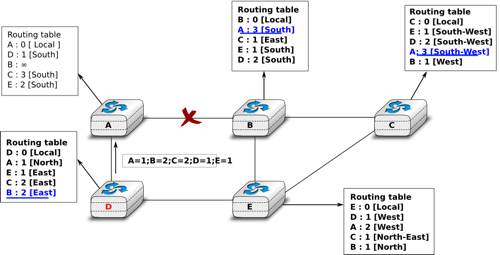
\includegraphics[scale=1.5]{dv-failure-2}
\end{figure}

Различные реализации дистанционно-векторного метода различаются, в частности,
оценками стоимости соединений в сети. Так, например, протокол RIP \cite{rip-rfc} просто
оценивает стоимость каждого соединения в 1, а IGRP \cite{igrp-patent} оценивает
стоимость соединений исходя из оценок задержки и пропускной способности.

Преимуществами дистанционно-векторных алгоритмов являются простота реализации и
низкие требования к памяти и вычислительной мощности. Недостатками же являются
низкая скорость распространения информации по сети и сложности с приспособлением
под изменяющуюся топологию (проблема count-to-infinity). Этих проблем
удается избежать при применении другого распространенного подхода - алгоритмов
на основе состояния канала связи. 

\subsection{Алгоритмы состояния канала связи}

В отличие от дистанционно-векторных алгоритмов, в алгоритмах состояния канала связи
(link-state) каждый узел сети хранит у себя модель всей сети в виде графа.
Рассмотрим шаги алгоритма подробнее:

\begin{itemize}
\item Каждый маршрутизатор периодически проверяет состояние соединений до
  соседей
\item При обнаружении обрыва какого-либо соединения алгоритм удаляет это
  соединение из собственного графа и рассылает соседям новую версию состояния
  соединений до них
\item Соседи обновляют собственные версии графов в соответствии с полученной
  информацией и пересылают сообщение дальше
\item Чтобы избежать зацикливания сообщений об обновлении состояния, каждое
  сообщение снабжается \textit{номером версии}. Маршрутизатор $n$ игнорирует
  сообщение от маршрутизатора $n$, если номер версии этого сообщения меньше или
  равен предыдущему.
\end{itemize}

\begin{figure}[!h]
  \caption{Иллюстрация работы link-state алгоритма}\label{ospf-img}
  \centering
  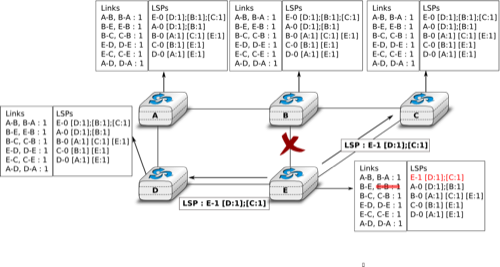
\includegraphics[scale=1.5]{ls-twoway}
\end{figure}

Имея информацию обо всей сети в целом, маршрутизатор может рассчитать кратчайшие
пути до всех остальных узлов. Обычно для этого используется алгоритм
Дейкстры \cite{dijkstra}. 

Link-state алгоритмы обладают способностью адаптироваться под изменения
топологии сети гораздо быстрее, чем distance-vector алгоритмы за счет
несколько более сложной реализации и чуть больших затрат по памяти и
вычислительной мощности. Это обуславливает то, что на данный момент именно
link-state протоколы, такие как OSPF \cite{ospf-rfc}, доминируют в сетевой
маршрутизации. Однако даже в решении задачи сетевой маршрутизации link-state
алгоритмы в чистом виде не лучшим образом адаптируются к повышению нагрузки в
сети. Рассматриваемые в дальнейшем другие алгоритмы, основанные на принципе
обучения с подкреплением, справляются с задачей адаптации к
изменчивой нагрузке лучше.

\subsection{Q-routing}\label{q-routing-desc}

Среди других подходов особый интерес представляют подходы на основе обучения с
подкреплением. Первым алгоритмом маршрутизации, основанным на этой идее, стал
алгоритм Q-routing \cite{q-routing-orig}. Принцип его работы таков:

\begin{itemize}
\item Каждый маршрутизатор $x$ хранит $Q_x(d, y)$ --- оценку минимального
  времени в пути до узла $d$, если следующим узлом на пути является сосед $y$.
  Очевидно, что $\forall y : Q_x(x, y) = 0$ 
\item Пакет, который необходимо доставить в узел $d$, отправляется соседу
  $y = \argmin\limits_{(x, y) \in E} Q_x(d, y)$
\item При получении пакета узел $y$ отправляет узлу $x$ время получения $t_r$ и
  собственную оценку оставшегося времени в пути
  $t = \min\limits_{(y, z) \in E} Q_y(d, z)$
\item Зная время отправления пакета $t_s$ и получив $t_r$ и $t$, узел $x$
  обновляет собственную оценку по формуле:
  $Q_x(d, y) = \alpha((t_r - t_s) + t - Q_x(d, y)) + Q_x(d, y)$,
  где $\alpha$ --- это learning rate, параметр алгоритма.
\end{itemize}

Было показано, что этот алгоритм способен хорошо адаптироваться к изменениям в
топологии сети и интенсивности трафика. Такие его модификации, как dual
Q-routing \cite{dual-q-routing} и predictive Q-routing \cite{predictive-q-routing}
демонстрируют еще более высокое качество маршрутизации. Однако по сравнению с
distance-vector или link-state методами данные алгоритмы используют гораздо
больше служебных сообщений (служебный пакет на каждую пересылку целевого
пакета), что ограничивает их применение в реальных высоконагруженных
компьютерных сетях.

Однако в задачах маршрутизации вне контекста компьютерных сетей это перестает
быть проблемой, так как целевые ``пакеты'' (чемоданы на конвейере, автомобили на
автостраде, etc.) и служебные сообщения в таких задачах являются объектами разной природы и
передаются по разным каналам, причем служебные сообщения по сравнению с целевыми
``пакетами'' доставляются мгновенно. Эти обстоятельства делают применение
алгоритмов обучения с подкреплением в таких задачах более привлекательным.

\subsection{Другие подходы}

Для полноты обзора приведем еще несколько примеров.

Идея использования нейросетей для решения задачи маршрутизации не нова. В
работах \cite{ali-nn-routing, araujo2001neural} для решения задачи поиска кратчайшего пути в графе
используются нейронные сети Хопфилда. Однако, эти исследования преследовали цель
ускорения вычисления кратчайшего пути за счет аппаратной реализации нейросети,
что кардинально отличается от цели текущей работы.

Еще одним интересным подходом является AntNet \cite{di1998antnet}. Это алгоритм,
построенный на идее исследования состояния сети с помощью специальных
пакетов-``агентов''. Алгоритм показал хорошие результаты в ходе исследований, но
не получил широкого применения, вероятно, в силу уже массового к тому времени
распространения link-state и distance-vector протоколов.

\subsection{Выводы по обзору существующих решений}\label{routing-overview-end}

Все рассмотренные алгоритмы маршрутизации были разработаны для
решения задачи маршрутизации именно в компьютерных сетях, но не для решения
задачи маршрутизации в общей формулировке. Таким образом, есть потребность в
разработке алгоритма, способного решать более общую задачу, что и является целью
данной работы.

\section{Применение обучения с подкреплением к задаче маршрутизации}

\subsection{Термины и понятия}

\textbf{Обучение с подкреплением} (reinforcement learning) --- вид машинного
обучения, в котором \textit{агент} (agent) каждый момент времени $t$
взаимодействует со \textit{средой} (environment), находящейся в
\textit{состоянии} (state) $s_t \in \mathcal{S}$ путем выбора
\textit{действия} (action) $a \in \mathcal{A}_{s_t}$ и получения
\textit{вознаграждения} (reward) $r_{t+1} \in \Bbb{R}$ c переходом в новое
\textit{состояние} $s_{t+1}$.

\begin{figure}[!h]
  \caption{Схема взаимодействия агента и среды в обучении с подкреплением}\label{rl-scheme}
  \centering
  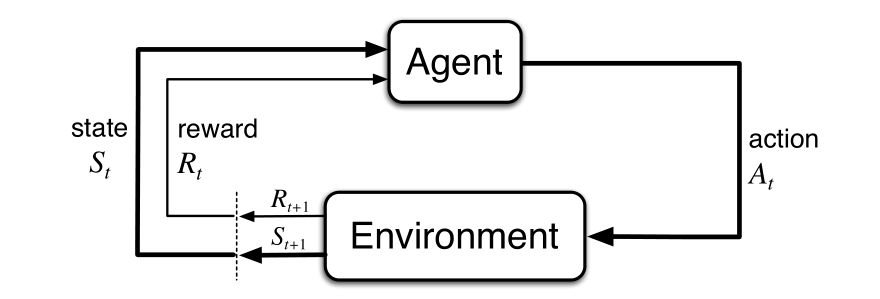
\includegraphics[scale=0.5]{rl-scheme}
\end{figure}

\textbf{Марковский процесс принятия решений} (Markov decision process, MDP) ---
это кортеж
$(\mathcal{S}, \mathcal{A}_s, P, R, \gamma)$, где

\begin{itemize}
\item $\mathcal{S}$ --- конечное множество состояний
\item $\mathcal{A}_s$ --- конечное множество действий, доступных из состояния
  $s$
\item $P(s' | s, a)$ --- вероятность того, что действие $a$ в состоянии $s$
  приведет к переходу в состояние $s'$ в следующий момент времени.
\item $R : \mathcal{S} \times \mathcal{A}_s \rightarrow \Bbb{R}$ ---
  вознаграждение за действия $a$ в состоянии $s$
\item $\gamma \in [0, 1]$ --- \textit{скидочный коэффициент} (discount factor),
  управляющий соотношением между важностью текущих вознаграждений и будущих вознаграждений.
\end{itemize}

\textbf{Оптимальной стратегией} для данного Марковского процесса принятия
решений называется такая функция выбора действий $\pi : \mathcal{S} \rightarrow \mathcal{A}_s$,
что взвешенная сумма вознаграждений $\sum\limits_{t=0}^{\infty} {\gamma^t
  R_{\pi(s_t)}(s_t, s_{t+1})}$ максимальна.

\textbf{Частично наблюдаемый Марковский процесс принятия решений} (Partially
observed Markov decision process, POMDP) --- это кортеж
$(\mathcal{S}, \mathcal{A}_s, P, R, \Omega, O, \gamma)$, где
\begin{itemize}
\item $\mathcal{S}$ --- конечное множество состояний
\item $\mathcal{A}_s$ --- конечное множество действий, доступных из состояния $s$
\item $P(s' | s, a)$ --- вероятность перехода из $s$ в $s'$ при выполнении
  действия $a$
\item $R : \mathcal{S} \times \mathcal{A}_s \rightarrow \Bbb{R}$ ---
  вознаграждение за действие $a$ в состоянии $s$.
\item $\Omega$ --- множество \textit{наблюдений}
\item $O(o | s', a)$ --- вероятность получения наблюдения $o$ при переходе в
  истинное состояние $s'$ в результате действия $a$. 
\end{itemize}

Определение оптимальной стратегии для частично наблюдаемого Марковского процесса
аналогично таковому для обычного.

Для Марковских процессов в условиях известности всех компонентов, включая $P$,
$R$ и $O$ существуют детерминированные методы нахождения оптимальной стратегии.
Однако найти оптимальную стратегию можно и в условиях неизвестности $P$, $R$ и $O$.

\textbf{Q-обучение} (Q-learning) \cite{q-learning-orig} --- это метод нахождения
оптимальной стратегии для Марковского процесса принятия решений, не требующий
информации о функции $R$ и распределении $P$. Метод заключается в оценке
\textit{функции полезности} (action-value function)
$Q(s,a)$. Функция полезности изменяется при каждом предпринятом действии $a$ с
переходом из состояния $s$ в $s'$ по следующей формуле:
\[
Q(s, a) = Q(s, a) + \alpha \left( r +
\gamma \cdot \max\limits_{a \in \mathcal{A}_{s'}} - Q(s', a) \right)
\]

Известно, что для любого конечного Марковского процесса принятия решений
Q-обучение находит оптимальную стратегию, т. е. $Q(s, a) \xrightarrow{t
  \rightarrow \infty} Q^*(s, a)$, и $\pi(s) = \argmax\limits_{a \in
  \mathcal{A}_s} {Q^*(s, a)}$ --- оптимальная стратегия.

\subsection{Формулировка задачи в терминах обучения с подкреплением}\label{rl-task-formulation}

Как было указано в \ref{routing-overview-end}, целью данной работы является
разработка алгоритма маршрутизации, способного решать эту задачу в обобщенной
постановке. Обобщенность постановки задачи делает разработку оптимального
детерминированного решения слишком сложной, вплоть до невозможности, что
приводит к идее разработки приближенного решения, например, с использованием
методов машинного обучения.

Однако эффективное использование обычного \textit{обучения с учителем} (supervised
learning) в данной задаче невозможно по следующим причинам:

\begin{itemize}
  \item Модель, использующая обучение с учителем, должна обучаться на
    достоверных примерах наблюдаемых состояний сети и соответствующих наилучших
    решениях о перенаправлении пакетов между узлами. Однако для получения
    подобных достоверных примеров, опять же, необходимо точное решение задачи,
    что в общем случае невозможно.
  \item Даже если удастся получить необходимые данные для обучения (например,
    с помощью некоторого \textit{централизованного} алгоритма), для покрытия
    всевозможных сценариев работы сети (при различной нагрузке, характере
    трафика, вариантов топологи и т. д.) потребуется очень большое количество данных.
\end{itemize}

При использовании же обучения с подкреплением обучающиеся агенты могут
подстраиваться под изменяющиеся условия в сети прямо во время работы, что
избавляет от вышеуказанных проблем, а также позволяет не вводить явным образом
многие скрытые параметры (такие как уровень нагрузки на сеть). Поэтому будем
формулировать задачу маршрутизации как задачу обучения с подкреплением.

К сожалению, сформулировать задачу маршрутизации в виде Марковского процесса
принятия решений довольно затруднительно. Попытаемся сформулировать ее
глобально. Пусть множество состояний $\mathcal{S}$ --- это Декартово произведение
состояний всех ребер и вершин в графе. Пусть также в состояние каждого ребра
(вершины) входит информация о всех пакетах, проходящих через это ребро
(обрабатывающихся в этой вершине). Пусть множество действий, доступных из
состояния $s \in \mathcal{S}$ $\mathcal{A}_s$ --- это множетво пар вида $(x,y)$,
где $x \in V$ --- это узел сети, имеющий в очереди пакет на обработку, а
$y \in \{V | (x, y) \in E\}$ --- один из его соседей. Таким образом, действие
интерпретируется как ``узел $x$ пересылает свой текущий пакет соседу $y$''.

У такой постановки задачи есть следующие проблемы:
\begin{enumerate}
\item Некоторые действия должны выполняться одновременно, а не одно за другим.
  Это можно формально обойти, сказав, что одновременно выполняющиеся действия
  $a_k, ... , a_{k+n}$ выполняются в последовательные моменты времени
  $t_k, ... , t_{k+n}$, либо изменив структуру множества действий
  $\mathcal{A}_s$: вместо пар $(x, y)$ рассматривать списки таких пар.
\item В любом случае невозможно узнать вознаграждение за действие $a_t$ сразу
  после перехода из состояния $s_t$ в $s_{t+1}$ --- вознаграждение за посылку
  пакета $p$ по ребру $e$ в вершину $v$ вычисляется как
  \[
  - \sum\limits_{t=t_k}^{t_{k+n}} {R_e(e, s_e^t, p)} -
  \sum\limits_{t=t_{k+n+1}}^{t_{k+m}} R_v(v, s_v^t, p)
  \]
  , где $t_k ... t_{k+n}$ --- моменты времени, в которые пакет проходил через
  ребро $e$, а $t_{k+n+1} ... t_{k+m}$ --- моменты времени, в которые пакет
  обрабатывался в узле $v$. (Суммы взяты с минусом, чтобы максимизация
  суммарного вознаграждения минимизировала суммарную стоимость путей пакетов).
  Это можно формально обойти, добавив в множество действий $\mathcal{A}_s$
  действия вида $a_e^p$ --- ``продолжить движение пакета
  $p$ по ребру $e$'' и $a_v^p$ --- ``продолжить продвижение пакета $p$ в очереди на
  обработку в узле $v$''. Однако такую формальную модель будет крайне сложно
  как-то применить на практике --- непонятно, как в какой-либо реальной задаче
  получить по отдельности стоимости вида $R_e(e, s_e^t, p)$ --- стоимости
  ``пребывания пакета $p$ на ребре $e$, которое находится в состоянии $s$.''
\end{enumerate}

Как можно видеть, несмотря на то, что формально процесс маршрутизации в сети
можно смоделировать как Марковский решающий процесс, оптимизация такой модели
невозможна с практической точки зрения как минимум потому, что в реальных
задачах полную информацию о состоянии всей сети в любой момент времени получить
нельзя.

Гораздо более логичным кажется рассмотреть задачу с точки зрения отдельного
маршрутизатора как обучающегося агента. Используя подход \textit{независимого
  Q-обучения} (independent Q-learning, IQL) \cite{tan1993multi}, скажем, что
маршрутизатор считает всю остальную часть сети как среду, с которой он
взаимодействует. Безусловно, маршрутизатору недоступна исчерпывающая информация
о состоянии всей сети, а только небольшая ее часть --- свое собственное
состояние, и, возможно, какая-то еще информация (о соединениях с соседями, о
самих соседях, возможно, что-то еще). Таким образом, кажется, что работу такого
агента можно смоделировать как частично наблюдаемый Марковский процесс. Однако и
здесь мы встречаемся с проблемой не мгновенного получения вознаграждения --- к
тому времени, как агент узнает от среды (а именно --- от соседа, которому он
послал пакет) финальную стоимость прохождения пакета до соседа, он успеет
сменить множество состояний. Более того, в такой постановке задачи состояние
$s_{t+1}$ почти никак не зависит от действия $a_t$. К тому же такая постановка
мотивирует маршрутизатор все время посылать пакеты по ребру наименьшей
стоимости, максимизируя таким образом свой собственный выигрыш, что явно не
оптимизирует суммарную стоимость пути пакета.

Однако все встает на свои места, если мы сделаем формальный трюк и в качестве
агента, взаимодействующего со средой, рассмотрим \textit{пакет}, двигающийся в
сети и стремящийся минимизировать суммарную стоимость своего пути. Пакет
рассматривает всю сеть как среду, а наблюдаемое состояние маршрутизатора, в
котором он находится, включая идентификатор этого маршрутизатора, как
собственное \textit{наблюдение}  $o_t \in \Omega$. С точки зрения пакета, во время
его движения по ребру ничего не происходит --- внутри маршрутизатора пакет
выбирает действие $a_t \in \mathcal{A}_o$ --- одного из соседей, в которого нужно
перейти, ``мгновенно'' перемещается в этого соседа с получением вознаграждения $r_t$,
равного суммарной стоимости этого перемещения, взятого с отрицательным знаком, и
получает новое наблюдение $o_{t+1} \in \Omega$ --- состояние нового маршрутизатора.

Как можно видеть, в такой формулировке задача хорошо моделируется как частично
наблюдаемый Марковский процесс. Для нахождения оптимальной стратегии в частично
наблюдаемом Марковском процессе также можно использовать принцип Q-обучения.
Несмотря на то, что в общем случае в POMDP Q-обучение не сходится к оптимальной
стратегии, на практике это дает хорошие результаты.

Запишем формулу Q-обучения для поставленной задачи:

\[
Q(o_t, a_t) = Q(o_t, a_t) + \alpha \left( r_t +
\gamma \cdot \max\limits_{a \in \mathcal{A}_{o_{t+1}}} Q(o_{t+1}, a) \right)
\]

Заметим, что путь пакета конечен, и нас интересует оптимизация его полной
стоимости. Поэтому в данной задаче будем считать, что $\gamma = 1$.

Eсли наблюдение состоит только из идентификатора текущего
узла, а вознаграждение является просто временем, потраченным пакетом на
перемещение, то эта формула вырождается в формулу, используемую алгоритмом
Q-routing (\ref{q-routing-desc}). Безусловно, на практике, как и в оригинальном
алгоритме Q-routing, сам пакет не является агентом, вычисляющим собственную
стратегию. Вместо этого на место каждого очередного пакета себя ставит
маршрутизатор.

Как уже было замечено, в общем случае множество наблюдений $\Omega$ может быть
очень большим или даже бесконечным, что обуславливает необходимость
аппроксимации функции $Q(o, a)$. Для этого можно использовать нейросети. В
следующей главе будут рассмотрены примеры применения нейросетей в задачах
обучения с подкреплением

\section{Обзор методов обучения нейросетей с подкреплением}\label{overview:nns}

Активные исследования в области обучения с подкреплением с использованием
нейросетей начались c публикации командой DeepMind алгоритма
DQN \cite{deepmind-dqn-orig}. Алгоритм показал способность эффективно обучаться
игре в классические видеоигры на эмуляторе Atari 2600. 

Алгоритм DQN базируется на методе Q-обучения. В качестве состояния нейросеть
получает на вход текущее изображение игрового экрана. Набор действий
соответствует возможному набору игровых действий.

\begin{figure}[!h]
  \caption{Устройство нейросети для приближения Q-функции}\label{dqn-scheme}
  \centering
  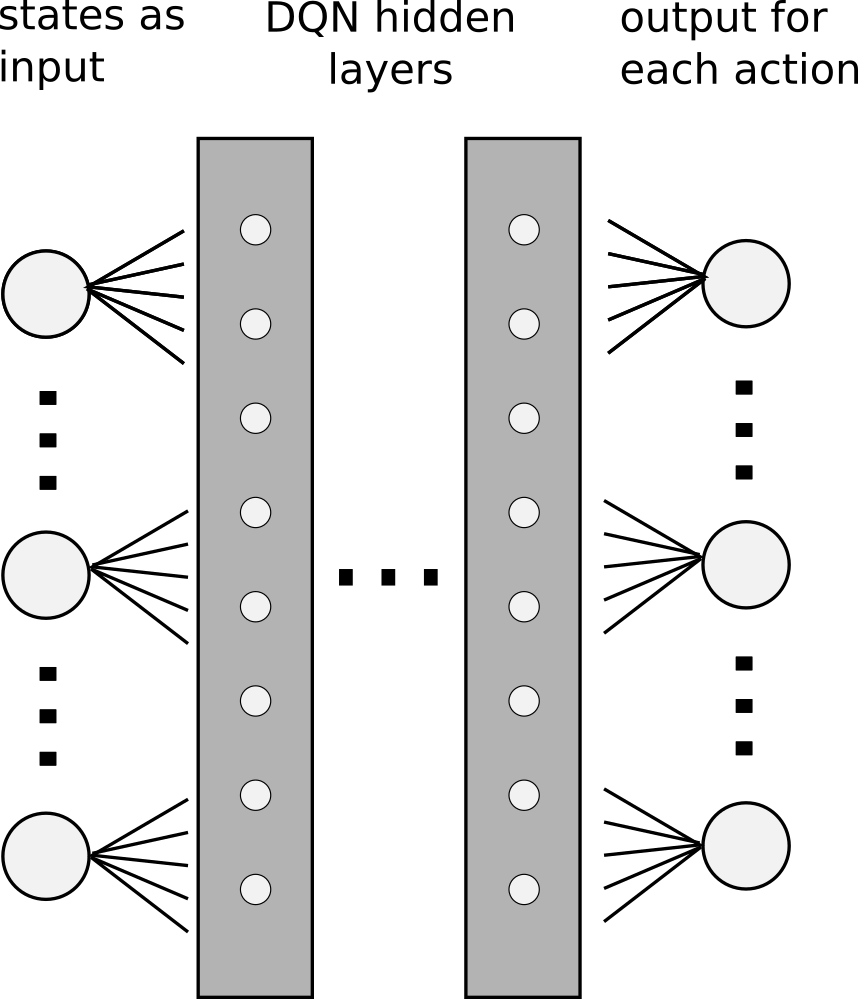
\includegraphics{dqn-scheme}
\end{figure}

Ключевой проблемой при использовании Q-обучения с нейросетями является то, что
метод Q-обучения в применении к Марковским процессам с бесконечным числом
состояний, вообще говоря, не сходится к оптимальной стратегии. Алгоритм DQN
борется с этим обстоятельством с помощью \textit{experience replay} --- буферa
из всех встреченных четверок $(s, a, r, s')$, где $s$ ---
начальное состояние, $a$ --- действие, предпринятое в этом состоянии, $r$ ---
полученное вознаграждение, $s'$ --- следующее состояние. Этот буфер работает как
``память'' нейросети: в каждый момент времени из буфера выбирается случайное
подмножество встреченных ситуаций, и нейросеть заново обучается на них,
``вспоминая'' игровой опыт. Кроме этого, для стабилизации процесса обучения в
алгоритме DQN использовалась \textit{целевая нейросеть} (target network) ---
дополнительная нейросеть, предоставляющая опорные оценки для основной сети и
копирующая ее состояние раз в $k$ шагов.

В дальнейшем было изобретено множество модификаций оригинального алгоритма DQN.
Из них можно выделить модификацию с использованием приоритизированного
experience replay \cite{schaul2015prioritized}. Идея приоритизированного
experience replay заключается в том, чтобы с большей вероятностью доставать из
буфера эпизоды, сильнее всего повлиявшие на процесс обучения -- т. е. те,
где нейросеть ошибалась в своих оценках Q-функции сильнее всего.
Также были разработаны такие модификации алгоритма, как Double
DQN \cite{van2016deep}, основанный на идее двойного
Q-обучения \cite{hasselt2010double} и Dueling DQN \cite{wang2015dueling},
основанный на идее оценки Q-функции как отдельных величин -- ценности состояния
$V(s)$ и преимущества действия $A(a)$.

Также в работе \cite{hausknecht2015deep} было показано, что добавление
LSTM-слоя \cite{hochreiter1997long} в архитектуру нейросети позволяет добиться
лучших результатов при оптимизации частично наблюдаемых Марковских процессов
благодаря сохранению информации о предыдущих наблюдениях в скрытом состоянии
рекуррентного слоя. В дальнейшем глубокие нейросети с рекуррентной архитектурой
показывали впечатляющие результаты в решении сложных задач, таких как игра
Doom \cite{lample2016playing}.

Одним из первых исследований по применению глубоких нейросетей в мультиагентной
среде является исследование \cite{tampuu2017multiagent}, в котором две нейросети
играли в игру Pong друг с другом. Но уже в работе \cite{foerster2016learning}
показано, что рекуррентные нейросети могут научиться пересылать друг другу сообщения для решения
совместных задач (в частности, в этом исследовании нейросети учились
разрабатывать совместную стратегию поведения для решения головоломки об узнике и
лампочке). На основе этой работы было проведено исследование
\cite{jorge2016learning}, в котором одна нейросеть обучалась
``задавать вопросы'' другой, чтобы по полученным ответам угадать, какое из
изображений ``загадала'' другая нейросеть.

\chapterconclusion

В главе 1 были рассмотрены существующие алгоритмы маршрутизации, их преимущества
и недостатки. Задача маршрутизации была сформулирована в терминах обучения с
подкреплением и были намечен подход к ее решению. Также был проведен обзор
современных методов глубокого обучения с подкреплением, в том числе в
мультиагентной среде.

\finishrelatedwork

\chapter{Описание разработанного алгоритма}

Идея алгоритма, который мы назовем \textit{DQN-routing}, заключается в
объединении метода Q-routing (\ref{q-routing-desc}) с обучением нейросетей.
Однако очевидно, что простая замена табличной Q-функции на нейросеть не даст
положительных результатов. Чтобы использовать преимущества нейросети, будут
применены такие подходы, как \textit{предобучение} и \textit{расширение
  наблюдаемого состояния}.

\section{Используемая архитектура нейросети}

Базовой частью любого текущего состояния $s$ (или, точнее \textit{наблюдения}
$o \in \Omega$) будем считать кортеж $(n, d, y_1 ... y_m)$, где $n$ --- это
идентификатор (номер) текущего узла, $d$ --- номер узла назначения текущего
пакета, а $y_1 ... y_m$ --- номера соседей текущего узла. Добавление номера
текущего узла позволит одной и той же нейросети работать в качестве роутера в
любом из узлов графа.

Чтобы избежать взаимозависимости оценок Q-функции для узлов с близкими номерами, будем
использовать \textit{унитарный код}, т. е. для сети с семью узлами номер 3 будет
кодироваться как 0010000, номер 5 --- как 0000100, и т. д. Для кодирования
множества соседей будем использовать тот же принцип, т. е. множество соседей 1,
3, 4 будет закодировано как 1011000. Таким образом, размер базового входного
состояния для нейросети составит $3n$, где $n$ --- количество узлов в сети.

\begin{figure}[!h]
  \caption{Feed-forward архитектура сети для графа из 5 узлов}\label{nn-pic-ff}
  \centering
  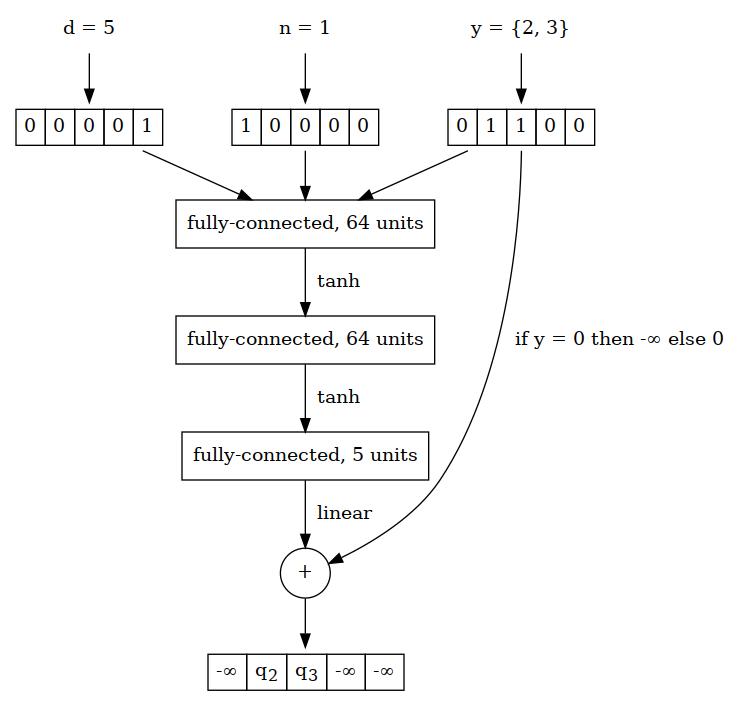
\includegraphics[scale=0.5]{nn-1}
\end{figure}

\begin{figure}[!h]
  \caption{Рекуррентная архитектура сети c ``памятью роутера'' для графа из 5
    узлов}\label{nn-pic-lstm-1}
  \centering
  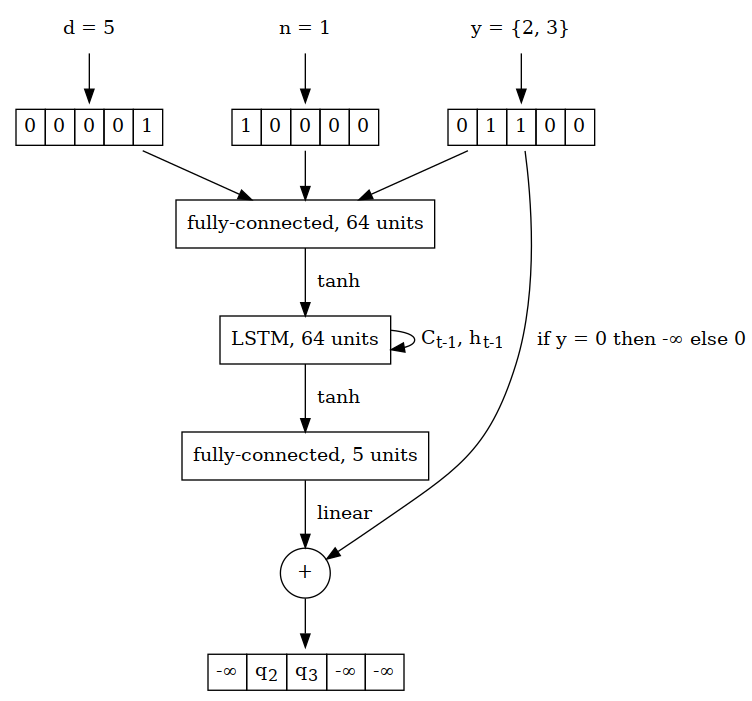
\includegraphics[scale=0.5]{nn-3}
\end{figure}

\begin{figure}[!h]
  \caption{Рекуррентная архитектура сети c ``памятью пакета'' для графа из 5
    узлов}\label{nn-pic-lstm-2}
  \centering
  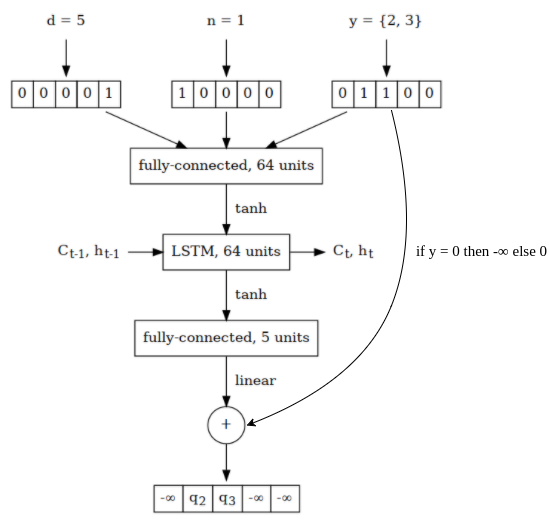
\includegraphics[scale=0.7]{nn-4-final}
\end{figure}

В работе будут рассматриваться три различные архитектуры нейросетей. Первой
архитектурой является обычная feed-forward нейросеть, имеющая 2 скрытых слоя с
гиперболическим тангенсом в качестве функции активации (рисунок
\ref{nn-pic-ff}). Другие две архитектуры нейросети
являются рекуррентными и имеют в качестве второго слоя
LSTM-ячейки \cite{hochreiter1997long}. Рекуррентные
архитектуры отличаются друг от друга характером передачи скрытого состояния.
Первый вариант (рисунок \ref{nn-pic-lstm-1}) работает как стандартная
рекуррентная сеть -- скрытое состояние $(C_t, h_t)$, полученное после обработки
очередного пакета $p_t$, сохраняется на маршрутизаторе и подается на скрытый
слой той же сети при обработке следующего пакета. Второй же вариант (рисунок
\ref{nn-pic-lstm-2}) работает иначе -- скрытое состояние $(C_t, h_t)$ LSTM-слоя
передается \textit{между} узлами графа \textit{вместе с пакетом}. При обработке
очередного пакета $p_t$ нейросеть подает содержащееся в нем скрытое состояние
$(C_t, h_t)$ на вход LSTM-слоя, и после обработки пакета передает новое скрытое
состояние $(C_{t+1}, h_{t+1})$ вместе с пакетом выбранному соседу. Таким
образом, можно сказать, что в первом случае скрытое состояние играет роль
``памяти маршрутизатора'', а во втором -- ``памяти пакета''.

Выходной слой для каждого из вариантов архитектуры состоит из $n$
нейронов с линейными функциями активации, где $i$-ый нейрон
соответствует $i$-ому узлу в сети. К выходам узлов, не являющихся соседями
текущего, отдельно прибавляется $-\infty$ (на практике --- большое отрицательное
число, например -1000000). Таким образом, на выходе нейросети образуются оценки
функции $Q(s, a)$ для всех действий $a$, где для действий, недоступных в текущем
состоянии (узлов, не являющихся соседями), $Q(s, a) = -\infty$.

Обучение нейросетей производится с помощью алгоритма оптимизации
RMSProp \cite{tieleman2012lecture}. Обоснование выбора именно этого алгоритма и
гиперболического тангенса в качестве функции активации приведено в приложении
\ref{apx:optimizers}

\section{Предобучение модели}

Как было указано в разделе \ref{rl-task-formulation}, мы будем моделировать
задачу маршрутизации как частично наблюдаемый Марковский процесс принятия
решений, рассматривая каждый пакет как независимого обучающегося агента,
взаимодействующего со средой, и впоследствии использовать метод Q-обучения для
оптимизации поведения агентов. Однако, как было отмечено в \ref{overview:nns},
Q-обучение с нейросетями в общем случае не сходится к оптимальному решению.
Бороться с этим с помощью experience replay и target network, как в оригинальном
алгоритме DQN, в мультиагентной среде не получается по причине
нестационарности среды: если каждый агент рассматривает всех остальных агентов
как часть среды, то поведение среды будет меняться вместе с поведением
обучающихся агентов, и старый опыт перестает быть релевантным. На графике
\ref{non-convergence} видно, что на практике нейросети действительно не могут
сойтись к оптимальному решению даже в условиях стабильной низкой нагрузки.

\begin{figure}[!h]
  \caption{Работа нейросетевой маршрутизации без
    предобучения}\label{non-convergence}
  \centering
  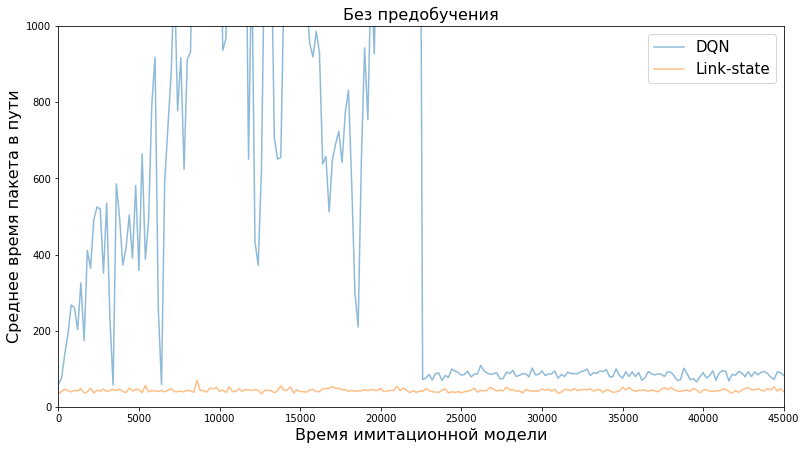
\includegraphics[scale=0.6]{non-convergence}
\end{figure}

Чтобы справиться с этой проблемой, будем использовать предварительное
\textit{обучение с учителем} (supervised learning). В качестве опорных данных
будут использованы данные работы алгоритма кратчайших путей в условиях низкой
нагрузки и равномерно распределенного трафика между узлами сети. В таких
условиях алгоритм кратчайших путей является оптимальным.

Предобучение feed-forward нейросети (рис. \ref{nn-pic-ff}) проводится на случайно
перемешанных данных, обучение рекуррентной нейросети с ``памятью роутера''
проводится на отсортированных по времени последовательностях эпизодов,
соответствующих одному роутеру, обучение рекуррентной нейросети с ``памятью
пакета'' проводится на последовательностях, соответствующих одному пакету.

Здесь стоит заметить, что, вообще говоря, не во всех вариантах постановки задачи
маршрутизации можно заранее вычислить стоимости прохождения пакета через ребра и
узлы сети даже в условиях низкой стационарной нагрузки (как, например, при
управлении конвейерной системой с учетом энергопотребления,
\ref{experiments:conveyors}). В таких случаях будем довольствоваться некоторыми
оптимистичными оценками на эти стоимости. Эксперименты показывают
(\ref{experiments:conveyors}), что в этом случае нейросети через некоторое время
подстраиваются под реальные стоимости и начинают работать оптимально.

Благодаря тому, что мы используем номер текущего узла как часть базового
состояния, мы можем предобучить одну нейросеть для работы во всех узлах сети,
что упростит процесс предобучения и сократит время на него.

\section{Расширение наблюдаемого состояния}

Интуитивно понятно, что чем больше релевантной информации мы используем для
оценки Q-функции, тем точнее в теории мы можем ее оценить. Очевидно, что
информация о текущей топологии в сети довольно важна для точности оценки. Эту
информацию мы можем эффективно передавать, используя link-state протокол.

\begin{figure}[!h]
  \caption{Архитектура сети с расширенным состоянием для графа из 5 узлов}\label{nn-pic-2}
  \centering
  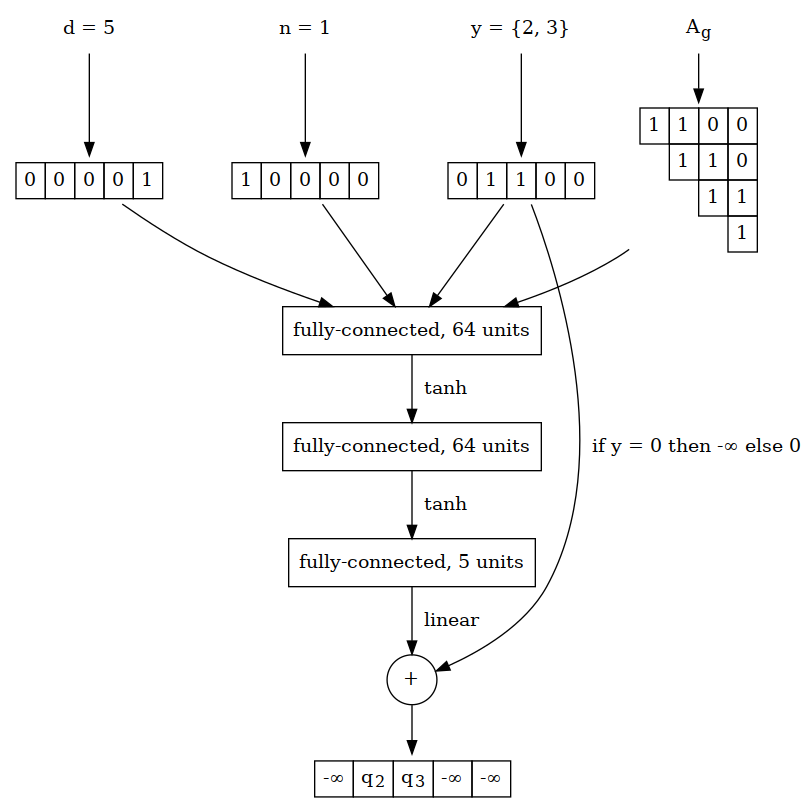
\includegraphics[scale=0.5]{nn-2}
\end{figure}

Имея версию текущей топологии графа, закодируем ее как \textit{матрицу
  смежности} и подадим на вход нейросети вместе с базовым состоянием в виде
вектора размера $n(n-1)/2$, где $n$ --- количество узлов в графе (рис.
\ref{nn-pic-2}). Таким образом мы получим возможность быстро реагировать на
обрывы и восстановление соединений. Эксперименты показывают
(\ref{experiments:simple/links}), что предобученная нейросеть с матрицей
смежности на входе и link-state протоколом в условиях низкой нагрузки и
изменяющейся топологии работает почти аналогично link-state алгоритму кратчайших
путей.

Кроме матрицы смежности, в наблюдаемое состояние сети можно добавить и другую
информацию. К примеру, при решении задачи управления конвейерной системой с
учетом энергопотребления (\ref{experiments:conveyors}) на вход нейросети
дополнительно будем подавать информацию о том, какие из соседних конвейеров в
данный момент находятся в рабочем состоянии (в виде вектора из нулей и единиц).

\section{Использование softmax-стратегии}\label{algo:softmax}

Алгоритмы обучения с подкреплением, особенно в нестационарных средах,
сталкиваются c проблемой застревания в локальном максимуме. Она заключается в
том, что алгоритм перестает менять свою стратегию, так как она ``кажется'' ему
наиболее выгодной, и не пробует никакие другие стратегии, хотя они на деле могут
оказаться выгоднее текущей. При решении задачи роутинга это чаще всего
проявляется в неоптимальности поведения алгоритма при переходе от высокой
нагрузки к низкой. Это является одним из основных недостатков оригинального
алгоритма Q-routing.

Частично решить эту проблему поможет \textit{softmax-стратегия}: выбор
следующего действия не детерминированно, а случайно, однако с распределением
вероятности, полученным применением к оценкам Q-функции функции
\textit{softmax}:
\[
\sigma(z)_j = \frac{e^{z_j}}{\sum_{k=1}^K {e^{z_k}}} \; \; \mathrm{for} \; \; j
= 1 \; .. \; K
\]

Это приводит к тому, что агент с некоторой вероятностью выбирает на очередном
шаге не самое оптимальное с его точки зрения действие, а что-то чуть менее
оптимальное, однако вероятность выбрать действие, оцениваемое как очень
невыгодное, крайне мала. Это помогает бороться с застреванием в локальном
максимуме с минимальным риском совершения очевидно невыгодных действий. В
приложении \ref{apx:softmax} продемонстрировано, как softmax-стратегия позволяет
алгоритму не застревать в неоптимальных решениях.

\chapter{Эксперименты}

\section{Эксперименты в модели компьютерной сети}\label{experiments:simple}

\subsection{Методология проведения экспериментов}\label{experiments:simple/desc}

Эксперименты проводились на имитационной модели сети из 10 узлов
(\ref{fig-simple-network}). Каждый роутер обрабатывает один пакет за 5 мс,
каждое соединение имеет задержку 10 мс и пропускную способность 1024 байт/с.
Каждый пакет имеет размер 1024 байт. Служебные сообщения (такие как сообщения о
вознаграждении от соседей) передаются по отдельному каналу, не зависящему от
времени имитационной модели. 

\begin{figure}[!h]
  \caption{Граф для тестов в модели компьютерной сети}\label{fig-simple-network}
  \centering
  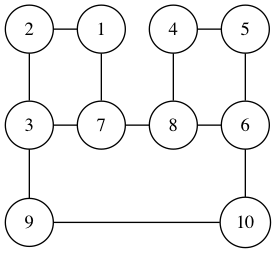
\includegraphics[scale=0.6]{graph-2.png}
\end{figure}

Нейросеть предварительно обучалась на эпизодах поведения роутеров, использующих
link-state протокол и алгоритм поиска кратчайшего пути (алгоритм Дейкстры).
Целевые оценки функции $Q(o, a)$ вычислялись как длины кратчайших путей от
текущего узла до узла назначения при условии прохождения через соседа $a$.

Работа предложенного алгоритма сравнивалась с работой link-state алгоритма и
алгоритма Q-routing. Такой выбор кандидатов для сравнения обусловлен тем, что
link-state алгоритмы являются доминирующими в сетевом роутинге, а алгоритм
Q-routing является идейным предком предложенного алгоритма.

Измерения проводились следующим образом:

\begin{itemize}
  \item Вычисляются средние стоимости пути пакетов по промежуткам времени в 500
    единиц времени имитационной модели.
  \item Порядок посылания пакетов при тестировании разных алгоритмов фиксируется
    путем фиксирования random seed
  \item Производится по 3 запуска эксперимента с различным random seed и
    полученные результаты усредняются
\end{itemize}

\subsection{Изменение топологии сети}\label{experiments:simple/links}

В этом сценарии при небольшой нагрузке в сети производился последовательный
обрыв соединений $(7, 8)$, $(1, 2)$ и $(5, 6)$ и последующее их восстановление в том
же порядке. Пакеты посылались между двумя половинами графа (между множествами
вершин $\{1, 2, 3, 7\}$ и $\{4, 5, 6, 8\}$).

\begin{figure}[!h]
  \caption{Изменение топологии сети (сравнение нейросетевых
    архитектур)}\label{experiment-link-failures-networks}
  \centering
  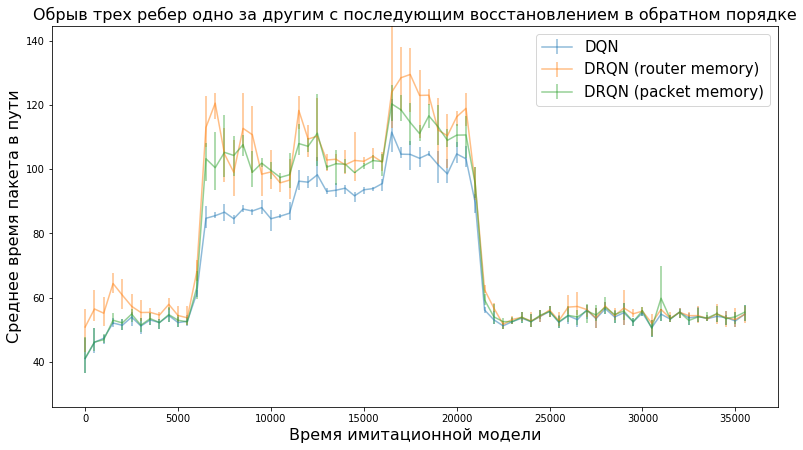
\includegraphics[scale=0.6]{experiment-link-failures-networks}
\end{figure}

Сначала были сравнены три рассматриваемые архитектуры нейросети: feed-forward,
рекуррентная с ``памятью роутера'' и рекуррентная с ``памятью пакета''. На
графике \ref{experiment-link-failures-networks} видно, что feed-forward
нейросети способны адаптироваться к изменению топологии лучше всего. Значит,
именно их мы будем сравнивать с алгоритмами link-state и Q-routing.

\begin{figure}[!h]
  \caption{Изменение топологии сети}\label{experiment-link-failures}
  \centering
  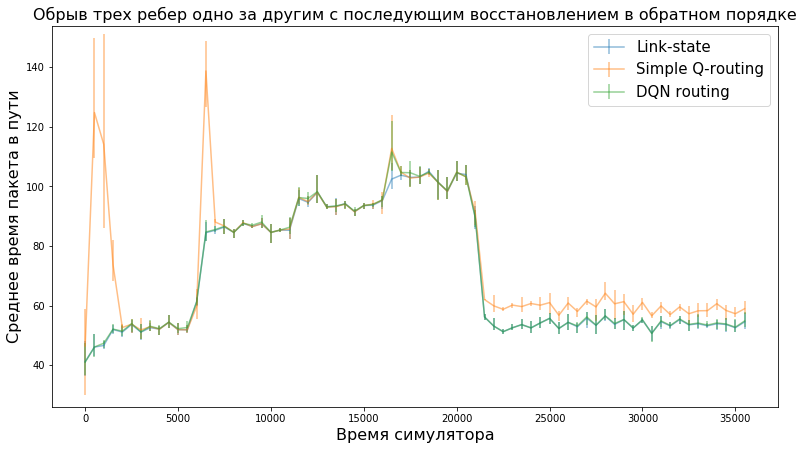
\includegraphics[scale=0.6]{experiment-link-failures}
\end{figure}

В условиях обрыва и восстановления соединений при низкой нагрузке работа
link-state алгоритма является оптимальной. На графике
\ref{experiment-link-failures} видно, что DQN-routing с feed-forward нейросетями
работает почти в точности так же, как и оптимальный в этой ситуации link-state
алгоритм, в то время как Q-routing не способен вернуться к оптимальному
поведению после восстановления всех соединений.

\subsection{Изменение интенсивности трафика}\label{experiments:simple/load}

В этом сценарии, как и в прошлом, пакеты перемещаются между двумя половинами
графа. Сначала пакеты посылаются раз в 10 мс, затем нагрузка резко возрастает --
пакеты посылаются с периодом 3.5 мс --, и в конце падает вновь.

\begin{figure}[!h]
  \caption{Увеличение и уменьшение нагрузки (сравнение нейросетевых
    архитектур)}\label{experiment-rnn-comparison}
  \centering
  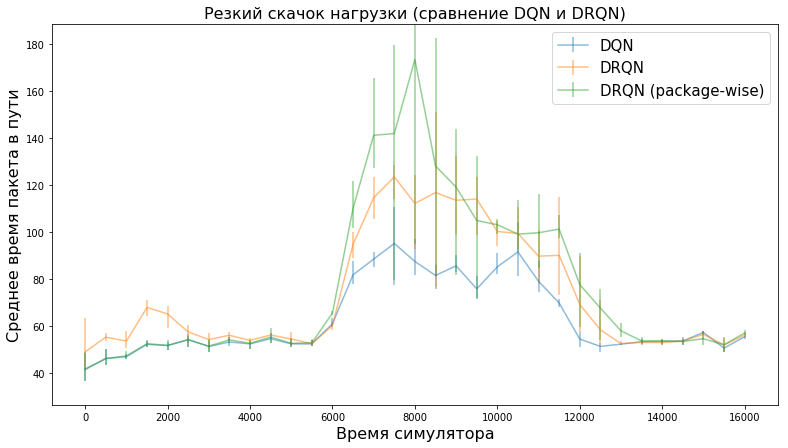
\includegraphics[scale=0.6]{experiment-rnn-comparison}
\end{figure}

График \ref{experiment-rnn-comparison} показывает, что и в этом случае
feed-forward нейросети приспосабливаются под меняющиеся условия наилучшим
образом, и именно их мы сравним с Q-routing и link-state алгоритмами.

\begin{figure}[!h]
  \caption{Увеличение и уменьшение нагрузки}\label{experiment-peak-load}
  \centering
  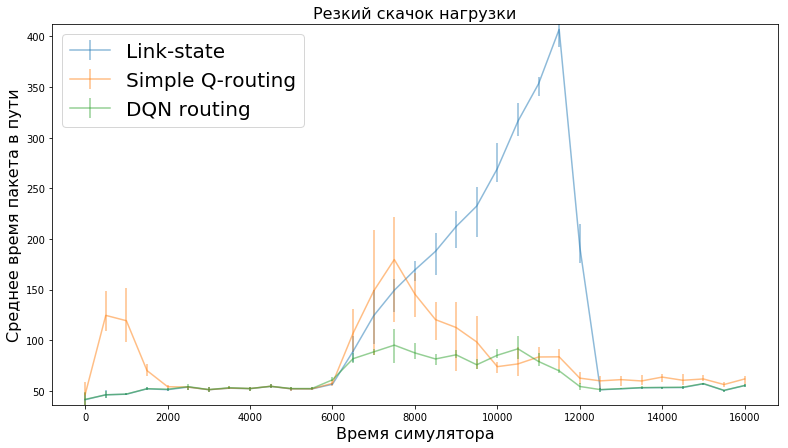
\includegraphics[scale=0.6]{experiment-peak-load}
\end{figure}

В условиях повышения нагрузки на сеть и перегрузки ``популярных'' роутеров,
через которые проходит большинство кратчайших путей (узлы 7 и 8 в графе
\ref{fig-simple-network}) алгоритм link-state не способен работать эффективно,
как видно на графике \ref{experiment-peak-load}. Алгоритмы Q-routing и
DQN-routing cпособны приспособиться и перенаправить часть трафика через узлы 9 и
10, однако Q-routing приспосабливается к повышению нагрузки медленнее, чем
DQN-routing, а также не способен вернуться к оптимальному поведению при снижении
нагрузки.

Как показывают эксперименты, DQN-routing превосходит алгоритмы link-state и
Q-routing в способности адаптироваться под разного рода изменения условий в
модели компьютерной сети.

\section{Эксперименты в модели системы транспортировки багажа}\label{experiments:conveyors}

\subsection{Методология проведения экспериментов}

Чтобы продемонстрировать работу алгоритма в более сложных условиях была
смоделирована система управления багажных конвейеров. Описание модели
приведено в приложении \ref{apx:conveyor-model}

В отличие от модели компьютерной сети, в модели конвейерной системы алгоритм
будет пытаться оптимизировать не только среднее время доставки пакета
(чемодана), но и \textit{энергопотребление} конвейеров. Оптимизация
энергопотребления заключается в том, чтобы использовать для доставки чемоданов
до точек назначения как можно меньше конвейеров.

Также как и в случае упрощенной модели сети, DQN-routing будет сравниваться с
Q-routing и link-state алгоритмом. Link-state алгоритм в качестве весов ребер
использует длины конвейерных секций. 

В алгоритме DQN-routing на вход нейросети будет дополнительно подаваться вектор
$w$ размера $n$ (где $n$ -- количество конвейеров в системе), в котором на $i$-ой
позиции стоит 0, если конвейер $i$ в данный момент находится в состоянии
ожидания, и 1 -- если он работает.

Предобучение и измерение результатов проводится так же, как и в модели
компьютерной сети (\ref{experiments:simple/desc}).

Эксперименты проводились на модели конвейерной сети из 14 конвейеров с 27
секциями в сумме, двумя входными вершинами и четырьмя выходными вершинами (рис.
\ref{test-conveyors}). Секции с 1 по 20 имеют длину 10 метров, с 21 по 27 - 2
метра. Энергопотребление каждого конвейера равно 1 киловатт, максимальная
скорость - 1 м/c.

\begin{figure}[!h]
  \caption{Модель конвейерной системы для тестов}\label{test-conveyors}
  \centering
  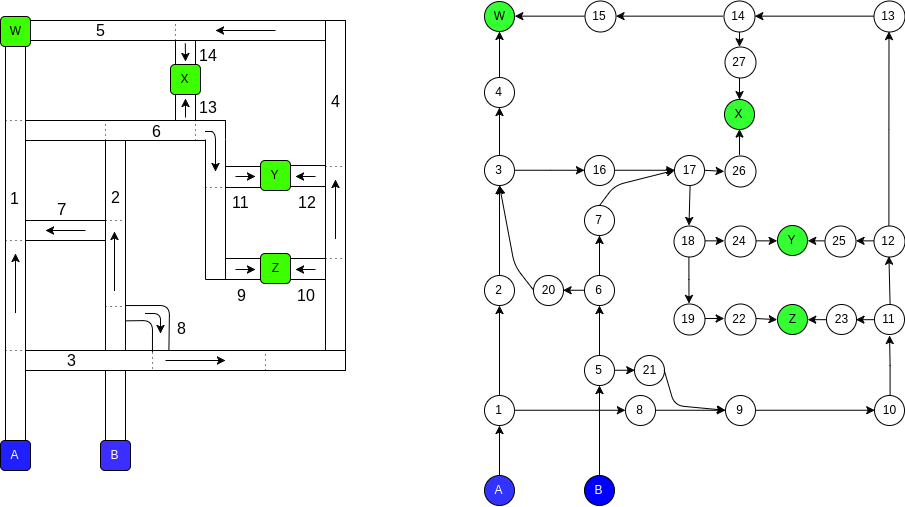
\includegraphics[scale=0.5]{test-conveyors}
\end{figure}

\subsection{Неравномерный поток до разных выходных вершин}\label{experiments:conveyors/altering-flow}

Как можно видеть на иллюстрации \ref{test-conveyors}, кратчайший путь от входов
до выходов W и X пролегает через конвейеры 1, 2, 7 и 6, а до выходов Y и Z --
через конвейеры 1, 2, 3 и 4. Однако до выходов Y и Z также можно попасть через
конвейер 6, не задействуя конвейеры 3 и 4. Если для нас важно оптимизировать
энергозатраты, то в условиях небольшого входящего потока чемоданов такая
стратегия является более предпочтительной.

\begin{figure}[!h]
  \caption{Время чемоданов в пути в условиях неравномерного потока до
    выходов (сравнение нейросетевых архитектур)}\label{experiment-conveyors-en1-time-nns}
  \centering
  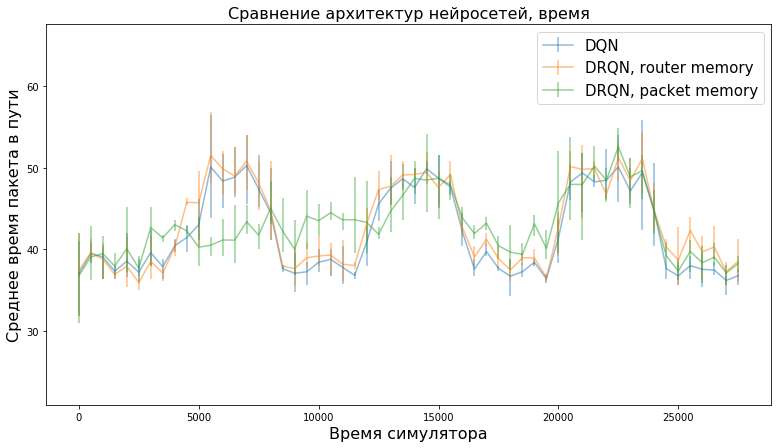
\includegraphics[scale=0.6]{experiment-conveyors-en1-time-nns}
\end{figure}

\begin{figure}[!h]
  \caption{Энергозатраты в условиях неравномерного потока до
    выходов (сравнение нейросетевых архитектур)}\label{experiment-conveyors-en1-energy-nns}
  \centering
  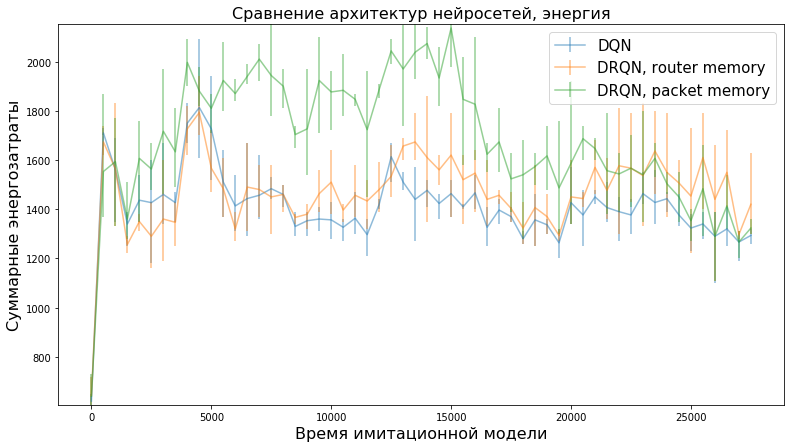
\includegraphics[scale=0.6]{experiment-conveyors-en1-energy-nns}
\end{figure}

В данном сценарии поток чемоданов попеременно идет либо только в выходы W и X,
либо во все четыре выхода сразу. Параметр важности экономии энергопотребления
$\alpha$ равен 1.

Вначале между собой были сравнены три рассматриваемые архитектуры нейросетей. На
графиках \ref{experiment-conveyors-en1-time-nns} и
\ref{experiment-conveyors-en1-energy-nns} видно, что feed-forward нейросети
лучше справляются как с оптимизацией времени работы, так и с оптимизацией
энергопотребления.

\begin{figure}[!h]
  \caption{Время чемоданов в пути в условиях неравномерного потока до
    выходов}\label{experiment-conveyors-en1-time}
  \centering
  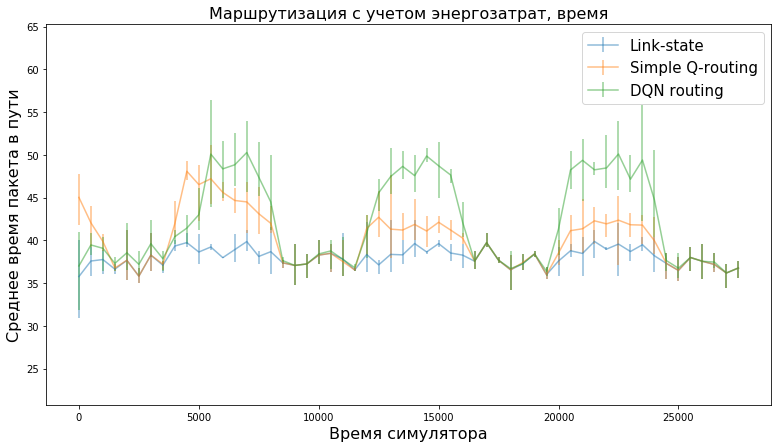
\includegraphics[scale=0.6]{experiment-conveyors-en1-time}
\end{figure}

\begin{figure}[!h]
  \caption{Энергозатраты в условиях неравномерного потока до
    выходов}\label{experiment-conveyors-en1-energy}
  \centering
  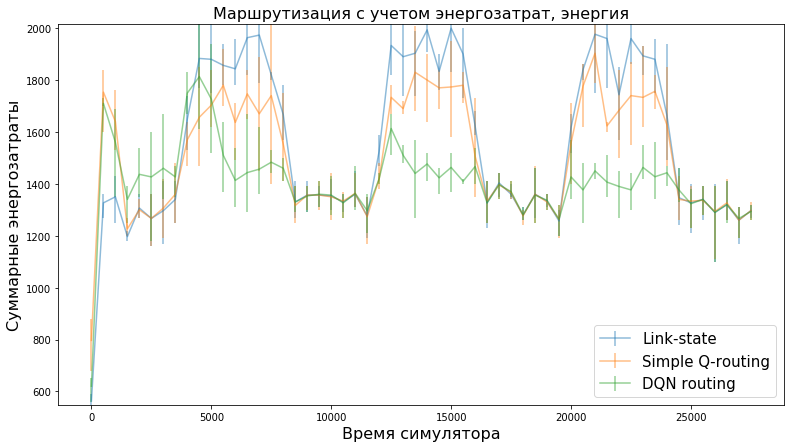
\includegraphics[scale=0.6]{experiment-conveyors-en1-energy}
\end{figure}

Далее DQN-routing с feed-forward нейросетями был сравнен с алгоритмами Q-routing
и link-state.
На графиках \ref{experiment-conveyors-en1-time} и
\ref{experiment-conveyors-en1-energy} видно, что алгоритм DQN-routing после
непродолжительного периода адаптации начинает работать заметно лучше алгоритмов
link-state и Q-routing с точки зрения экономии энергии, жертвуя средним временем
доставки чемодана. Это происходит благодаря тому, что нейросети обладают
информацией о том, какой из соседей на данный момент работает, а какой -- нет.

\subsection{Плавное повышение нагрузки}\label{experiments:conveyors/load}

Первая половина этого сценария повторяет предыдущий -- поток попеременно идет то
во все выходы, то только в выходы W и X. Во второй половине сценария частота
появления чемоданов на входах возрастает в 2 раза и продолжает плавно расти. В
этом сценарии будет продемонстрировано влияние коэффциента важности экономии
энергопотребления $\alpha$.

Так как этот сценарий по сути довольно похож на предыдущий, здесь мы рассмотрим
только feed-forward архитектуру нейросетей как архитектуру, показавшую наилучшие
результаты в предыдущем сценарии.

\begin{figure}[!h]
  \caption{Время чемоданов в пути в условиях плавного повышения нагрузки,
    $\alpha = 1$}\label{experiment-conveyors-a1-time}
  \centering
  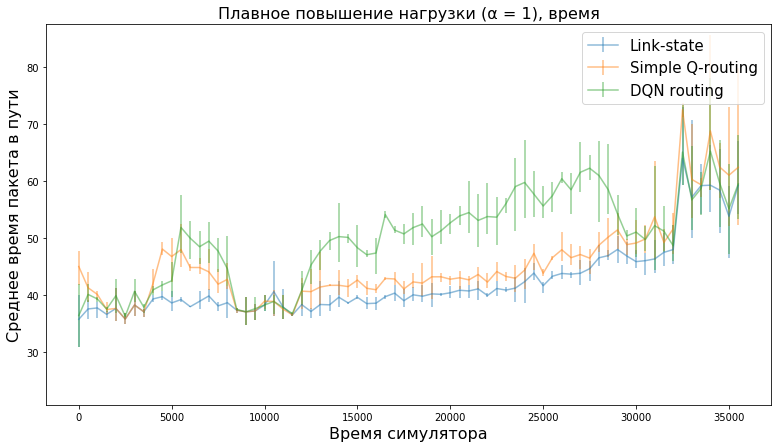
\includegraphics[scale=0.6]{experiment-conveyors-a1-time}
\end{figure}

\begin{figure}[!h]
  \caption{Энергозатраты в условиях плавного повышения нагрузки, $\alpha =
    1$}\label{experiment-conveyors-a1-energy}
  \centering
  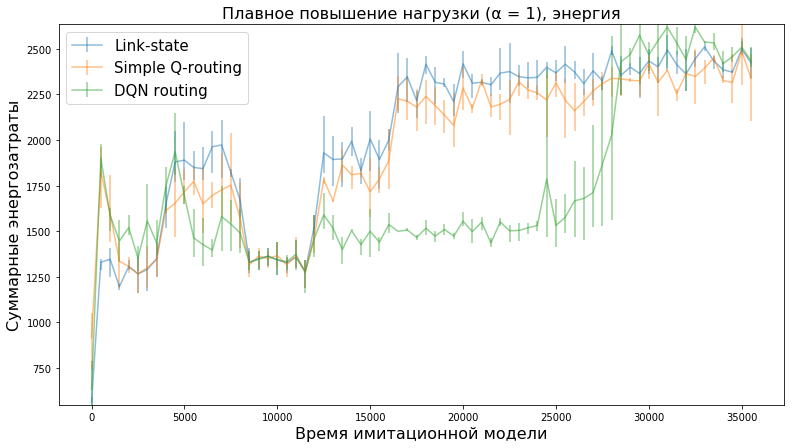
\includegraphics[scale=0.6]{experiment-conveyors-a1-energy}
\end{figure}

На графиках \ref{experiment-conveyors-a1-time} и
\ref{experiment-conveyors-a1-energy} видно, что алгоритм DQN-routing долгое
время отдает предпочтение экономии энергии, но ближе к концу сценария среднее
время чемодана в пути становится слишком высоким, и алгоритм начинает
использовать путь по конвейерам 3 и 4.

\begin{figure}[!h]
  \caption{Время чемоданов в пути в условиях плавного повышения нагрузки,
    $\alpha = 0.6$}\label{experiment-conveyors-a06-time}
  \centering
  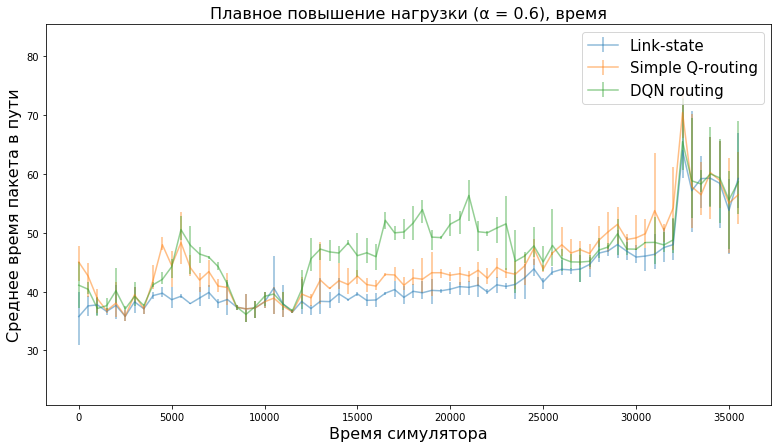
\includegraphics[scale=0.6]{experiment-conveyors-a06-time}
\end{figure}

\begin{figure}[!h]
  \caption{Энергозатраты в условиях плавного повышения нагрузки, $\alpha =
    0.6$}\label{experiment-conveyors-a06-energy}
  \centering
  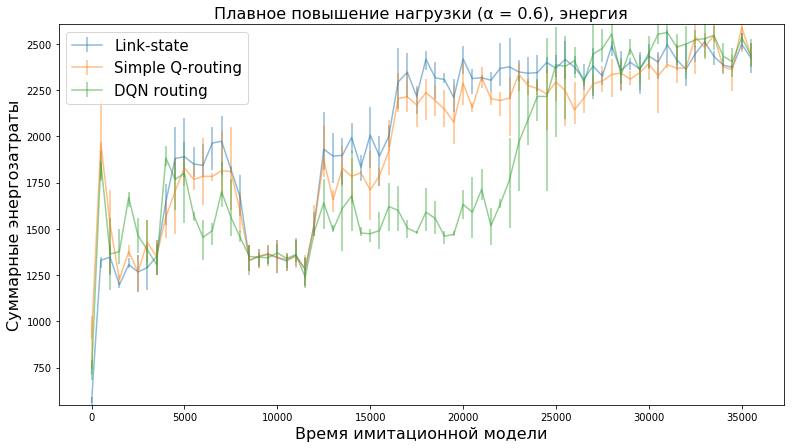
\includegraphics[scale=0.6]{experiment-conveyors-a06-energy}
\end{figure}

Графики \ref{experiment-conveyors-a06-time} и
\ref{experiment-conveyors-a06-energy} показывают, что при понижении коэффициента
важности энергопотребления $\alpha$ c $1$ до $0.6$ DQN-routing начинает
использовать конвейеры 3 и 4 раньше.

%% Макрос для заключения. Совместим со старым стилевиком.
\startconclusionpage

В данной работе был представлен новый алгоритм решения задачи маршрутизации на основе
обучения с подкреплением с использованием нейронных сетей --
\textit{DQN-routing}. Были разработаны имитационные модели компьютерной сети и
системы управления багажными конвейерами. Алгоритм сравнивался с link-state
алгоритмом кратчайших путей, так как link-state алгоритмы на данный момент
являются наиболее широко используемыми алгоритмами маршрутизации, и алгоритмом
Q-routing, также основанным на идее обучения с подкреплением.

Как в задаче сетевого роутинга, так и в задаче управления конвейерами алгоритм
превзошел link-state алгоритм и Q-routing по качеству работы в изменяющихся
условиях среды. Было показано, что алгоритм может решать задачи с разнородными
условиями, требуя при этом лишь незначительных и однотипных модификаций.
Таким образом, существует перспектива применения алгоритма также и для других
задач, не рассмотренных в данной работе.

\printmainbibliography

\appendix

\chapter{Описание разработанных имитационных моделей}\label{apx:simulators}

\section{Описание модели компьютерной сети}\label{apx:network-model}

В модели компьютерной сети оптимизируемой функцией является среднее время пакета в
пути от источника то узла назначения. Вознаграждение $r$ за действие $y$
(перенаправление пакета в соседа $y$) вычисляется как время между отправкой
пакета $t_{start}$ и временем его обработки в соседнем роутере $t_{finish}$.

Каждый роутер $n$ может обработать один пакет раз в $t_d^n$ единиц времени имитационной
модели (будем для удобства считать, что время имитационной модели измеряется в
\textit{миллисекундах}). Если пакет приходит в роутер до того, как обработается
предыдущий, он остается в очереди на обработку, размер очереди не ограничен.

Соединение между роутерами $u$ и $v$ имеет свойства \textit{задержки} $l_{uv}$ и
\textit{пропускной способности} $c_{uv}$. Входящее и исходящее соединения
независимы, в общем случае $l_{uv} \neq l_{vu}$ и $c_{uv} \neq c_{vu}$.

Каждый пакет $p$ имеет определенный \textit{размер} $s_p$.
Считается, что по соединению в каждый момент времени передается один пакет, и
пакет не может начать передаваться до того, как предыдущий пакет полностью
покинет роутер. Пакет загружается в канал связи за время $s_p / c_{uv}$ и
достигает соседнего роутера за время $l_{uv}$. Таким образом, полное время между
принятием решения об отправке пакета $p$ из роутера $u$ в роутер $v$ и его
обработкой на роутере $v$ составляет $s_p / c_{uv} + l_{uv} + t_{queue}$, где
$t_{queue}$ -- время ожидания пакета в очереди роутера $v$ (возможно, нулевое).

\section{Описание модели конвейерной системы}\label{apx:conveyor-model}

Система багажных конвейеров моделируется как ориентированный граф. Каждый
конвейер разбивается на \textit{секции} --- участки между примыкающими или
ответвляющимися конвейерами. Каждой \textit{секции} соответствует один узел в
графе; таким образом, один конвейер в общем случае моделируется несколькими
узлами в сети (рис. \ref{conveyors-illustration}).

\begin{figure}[!h]
  \caption{Участок конвейерной сети и соответствующий участок
    графа}\label{conveyors-illustration}
  \centering
  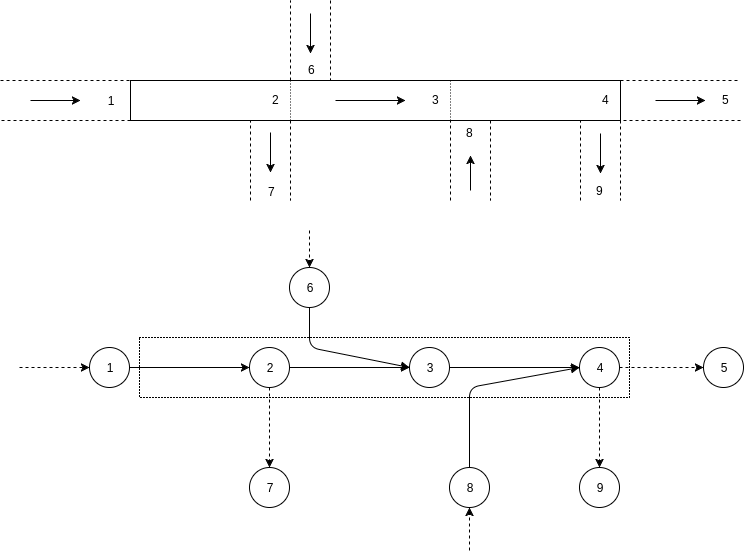
\includegraphics[scale=0.6]{belt-illustration}
\end{figure}

Для каждой секции конвейера определена ее \textit{длина}. Каждый конвейер
обладает такими свойствами как \textit{максимальная скорость} $v$,
\textit{энергопотребление за единицу времени} $e_t$ и \textit{задержка перед
  остановкой} $t_d$. Для удобства пояснения будем считать, что единицей длины
является \textit{метр}, единицей времени является \textit{секунда}, а единицей
измерения энергопотребления за единицу времени является \textit{киловатт}.

Энергопотребление конвейеров моделируется следующим образом. Каждый конвейер
находится либо в состоянии \textit{работы}, либо в состоянии \textit{ожидания}.
В состоянии работы конвейер потребляет $e_t$ энергии в секунду, в состоянии
ожидания конвейер энергии не потребляет. Изначально все конвейеры находятся в
состоянии ожидания. Конвейер переходит из состояния работы в состояние ожидания
тогда, когда на него перенаправляется чемодан, и возвращается в состояние
ожидания спустя $t_d$ секунд после того как на нем не остается ни одного
чемодана. При переходе из состояния работы в состояние ожидания и наоборот
конвейер сообщает об этом всем своим соседям. Каждый конвейер хранит информацию
о том, в каком состоянии находятся его соседи.

Конвейер принимает решение о том, куда перенаправить очередной чемодан из секции
$n$ в тот момент, когда чемодан въезжает на эту секцию. Таким образом, для
каждого чемодана, находящегося на секции $n$, известна следующая секция на его пути.

\textit{Текущий выходной поток} $f_o^{n,m}$ секции $n$ в направлении секции
$m$ определяется как среднее количество чемоданов, покидающих секцию за единицу
времени. В каждый момент времени текущий выходной поток секции вычисляется по
формуле $f_o^n = \frac{k_{n,m} v_n}{l_n}$, где $k_{n,m}$ -- текущее количество чемоданов
на секции $n$, направляющихся в секцию $m$, $l_n$ -- длина секции, и $v_n$ --
текущая скорость конвейера. Текущий выходной поток конвейера равен текущему
выходному потоку его последней секции. Будем считать, что чемоданы имеют длину в
1 метр и во избежание заторов необходимо оставлять между ними зазоры не менее
метра. Таким образом, максимальное количество чемоданов, которое может
находиться на секции конвейера, равно $l_n/2$. Следовательно, \textit{текущий максимальный поток} $f_m^n$, который может
проходить через секцию, равен $\frac{v_n}{2l_n}$.

\textit{Остаточный входной поток} $f_r^n$ секции $n$ определяется как дополнительный поток
чемоданов, который может принять секция с примыкающего сбоку конвейера в данный момент
времени. То есть если секция $n$ следует за секцией $m$ в рамках одного
конвейера, то $f_r^n = f_m^n - f_o^m$. Если секция $n$ является у конвейера
первой, то $f_r^n = f_m^n$.

При изменении величин остаточных входных потоков секций (вследствие изменения
скорости или входящих потоков от соседей) конвейер сообщает новые значения этих
величин своим соседям. Если остаточный поток секции $n$ ($f_r^n$) оказывается меньше, чем
соответствующее значение $f_o^{m,n}$ выходного потока секции $m$ соседнего конвейера, то
соседний конвейер снижает свою текущую скорость $v$, чтобы снизить выходной
поток до уровня остаточного потока примыкающей секции.

Среди вершин графа выделены \textit{входные} вершины и \textit{выходные}
вершины. Входные вершины не имеют входящих ребер и имеют только одно исходящее
ребро. Выходные вершины не имеют исходящих ребер и имеют одно или несколько
входящих. Каждый чемодан появляется на входной вершине и направляется в одну из
выходных. Для простоты будем считать, что любая выходная вершина способна
принимать входящий поток любой величины. Также будем считать, что если исходящий
поток из входной вершины превышает текущий остаточный поток примыкающей к ней
секции, то чемоданы накапливаются в очереди неограниченного размера.

Стоимость пути чемодана $p$ вычисляется по формуле $C_p = t_p + \alpha e_p$, где
$t_p$ -- это время чемодана в пути, $e_p$ -- энергозатраты на перемещение чемодана,
а $\alpha$ -- константный параметр, характеризующий ``важность'' экономии
энергии по сравнению со скоростью доставки чемоданов.

Остановимся подробнее на вычислении величины $e_p$. Суммарные энергозатраты на
перемещение чемодана складываются из энергозатрат каждого отдельного конвейера
$k$ на пути чемодана: $e_p = \sum\limits_{k \in path(p)} {e_p^k}$.
Величины $e_p^k$ считаются как $e_p^k = t_p^k \cdot e_t^k$, где $e_t^k$ --
энергопотребление конвейера $k$ за единицу времени, а
$t_p^k = (t_l^{k,p} + t_d^k) - t_s^k$, где $t_l^p$ -- время покидания конвейера $k$
чемоданом $p$, $t_d^k$ -- задержка конвейера $k$ перед остановкой, а $t_s^k$ --
ожидаемое время остановки конвейера перед тем, как чемодан покинул его. Если в
момент захода чемодана на конвейер $t_e$ конвейер находится в состоянии
ожидания, то считаем, что $t_s^k = t_e$. Величина $t_s^k$ обновляется с каждым
очередным чемоданом $p$, покидающим конвейер, по формуле
$t_s^k = t_l^{k,p} + t_d^k$. Таким образом, величина $t_p^k$ имеет смысл
``насколько дольше конвейер $k$ проработал из-за того, что по нему проехал
чемодан $p$''

Заметим, что при таком определении энергозатрат на перемещение чемодана
суммарные энергозатраты на все чемоданы совпадают с суммарными энергозатратами
всех конвейеров:
\[
\sum\limits_p {e_p} = \sum\limits_p {\sum\limits_{k \in path(p)} {t_p^k \cdot
    e_t^k}} = \sum\limits_k {e_t^k \sum\limits_{\{p | k \in path(p)\}} {t_p^k}}
= \sum\limits_k {e_t^k \cdot t^k} 
\],
где $t_k$ -- суммарное время работы конвейера $k$.

Заметим, что если мы будем вычислять величину $e_p^n$ отдельно для каждой
\textit{секции} $n$ конвейера $k$, сохранив общее для всех секций значение
$t_s^k$, то ничего не изменится. Действительно, мы можем рассматривать секции
конвейера как отдельные конвейеры, но запускающиеся и останавливающиеся в одно и
то же время. Если покинув секцию $n$ чемодан добавил к ожидаемому времени работы
конвейера $t_p^n$ и перешел в следующую секцию $m$ этого же конвейера, при покидании
следующей секции он добавит к ожидаемому времени работы $t_p^m$, и так далее,
пока чемодан не покинет конвейер. Очевидно, что $t_p^k = \sum_{n \in k} t_p^n$,
и значит $e_p^k = \sum_{n \in k} e_p^n$. 

Используемые в алгоритмах Q-routing и DQN-routing вознаграждения за действие $a$
-- перенаправление пакета в секцию $n$ -- в представленной модели имеют вид
$r =t^n + \alpha e_p^n$, где $t^n$ -- время на путь чемодана вдоль секции, а $e_p^n$
-- определенные выше энергозатраты на провоз чемодана вдоль секции.

Так как в отличие от модели компьютерной сети в данной модели граф является
ориентированным и (вообще говоря) не сильно связным, существует вероятность
приведения чемодана туда, откуда он не сможет добраться до нужной выходной
вершины. Чтобы избежать этого, при тестировании каждого алгоритма
используется link-state протокол, чтобы иметь информацию о том, из каких секций
конвейерной системы существует путь до требуемого выхода, а из каких -- нет, и
выбор следующей вершины на пути чемодана в алгоритмах DQN-routing и Q-routing
осуществляется только из тех соседней, из которых путь существует.

\chapter{Промежуточные результаты исследования}

\section{Выбор алгоритма оптимизации и функции активации для feed-forward нейросети}\label{apx:optimizers}

Было рассмотрено четыре популярных алгоритма оптимизации для нейросетей с адаптивным
шагом обучения: RMSProp \cite{tieleman2012lecture},
AdaDelta \cite{zeiler2012adadelta}, AdaGrad \cite{duchi2011adaptive} и
Adam \cite{kingma2014adam}. Также были проведены сравнения трех функций
активации: сигмоиды, гиперболического тангенса и ReLU.

Сначала алгоритмы были сравнены на этапе предобучения нейросети. Использовался
набор данных для упрощенной модели сети (\ref{experiments:simple}), обучение
велось на протяжении 20 эпох. На графиках
\ref{experiment-optimizers-pretrain-relu} и
\ref{experiment-optimizers-pretrain-tanh} видно, что AdaDelta и AdaGrad не
справляются с задачей, в то время как RMSProp и Adam показывают приблизительно
одинаковую эффективность.

\begin{figure}[!h]
  \caption{Сравнение алгоритмов оптимизации по эффективности
    предобучения, ReLU слои}\label{experiment-optimizers-pretrain-relu}
  \centering
  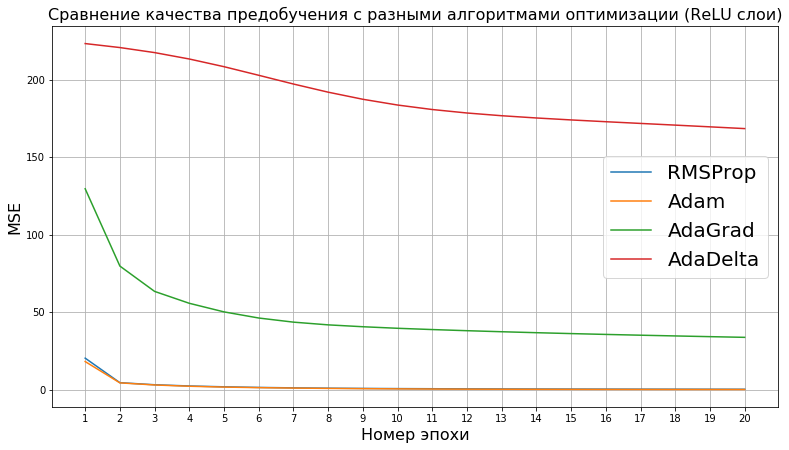
\includegraphics[scale=0.6]{experiment-optimizers-pretrain-relu}
\end{figure}

\begin{figure}[!h]
  \caption{Сравнение алгоритмов оптимизации по эффективности
    предобучения, tanh слои}\label{experiment-optimizers-pretrain-tanh}
  \centering
  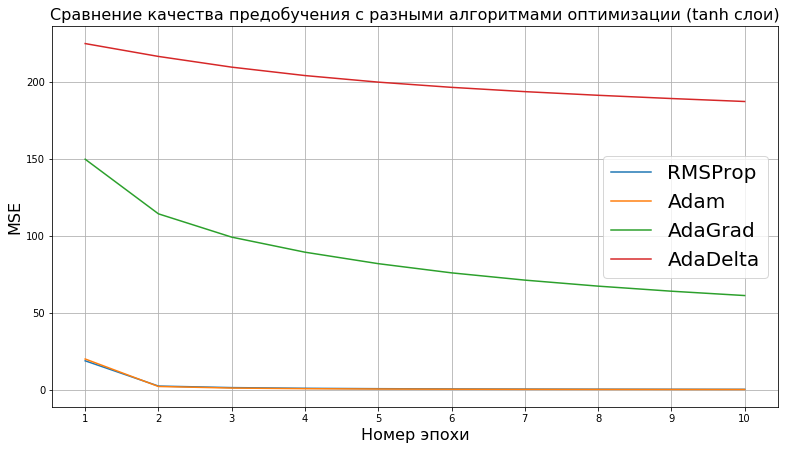
\includegraphics[scale=0.6]{experiment-optimizers-pretrain-tanh}
\end{figure}

Далее было проведено сравнение алгоритмов Adam и RMSProp с применением различных
функций активации. На графике
\ref{experiment-optimizers-pretrain-adam-vs-rmsprop} видно, что Adam во всех
случаях предобучается немного быстрее, нейросети на основе гиперболического
тангенса предобучаются быстрее всего, а на основе ReLU --- медленнее всего.

\begin{figure}[!h]
  \caption{Сравнение Adam и RMSProp по эффективности предобучения с различными
    функциями активации}\label{experiment-optimizers-pretrain-adam-vs-rmsprop}
  \centering
  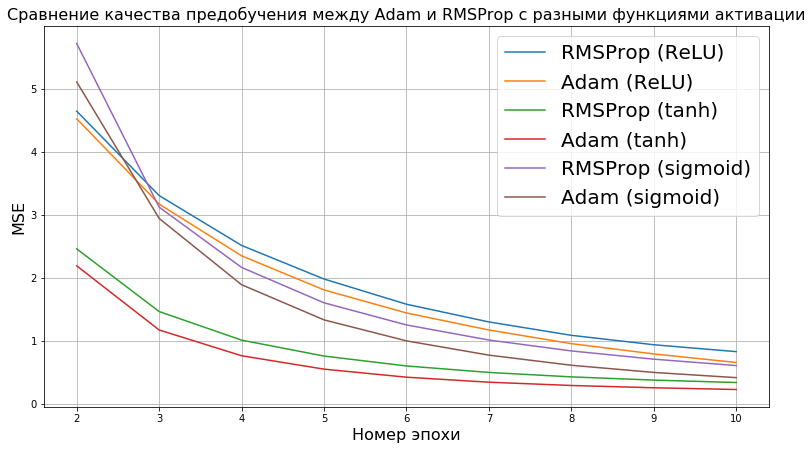
\includegraphics[scale=0.6]{experiment-optimizers-pretrain-adam-vs-rmsprop}
\end{figure}

Далее был поставлен эксперимент по сравнению качества Adam и RMSProp c tanh
активацией при работе внутри имитационной модели. Было установлено
(\ref{experiment-adam-failure}), что Adam не способен адекватно работать в
условиях изменяющейся нагрузки в сети, в отличие от RMSProp.

\begin{figure}[!h]
  \caption{Сравнение Adam и RMSProp по эффективности работы в
    имитационной модели}\label{experiment-adam-failure}
  \centering
  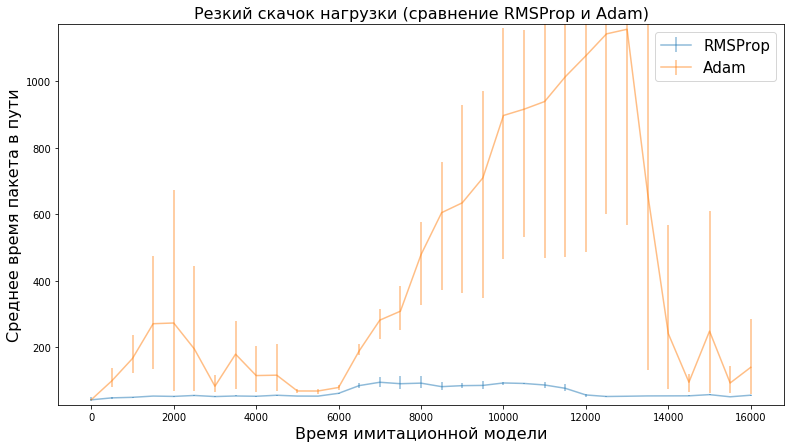
\includegraphics[scale=0.6]{experiment-adam-failure}
\end{figure}

На последнем этапе было сравнено качество работы RMSProp с различными фукнциями
активации при изменении нагрузки на сеть. График
\ref{experiment-activations-launch} показывает, что выбор функции активации
существенно не влияет на адаптивность к изменению нагрузки. Так как при этом
нейросети, использующие гиперболический тангенс, показали наилучшую скорость
предобучения (график \ref{experiment-optimizers-pretrain-adam-vs-rmsprop}), в
качестве используемой функции активации был выбран именно гиперболический
тангенс.

\begin{figure}[!h]
  \caption{Сравнение функций активации по эффективности работы в
    имитационной модели}\label{experiment-activations-launch}
  \centering
  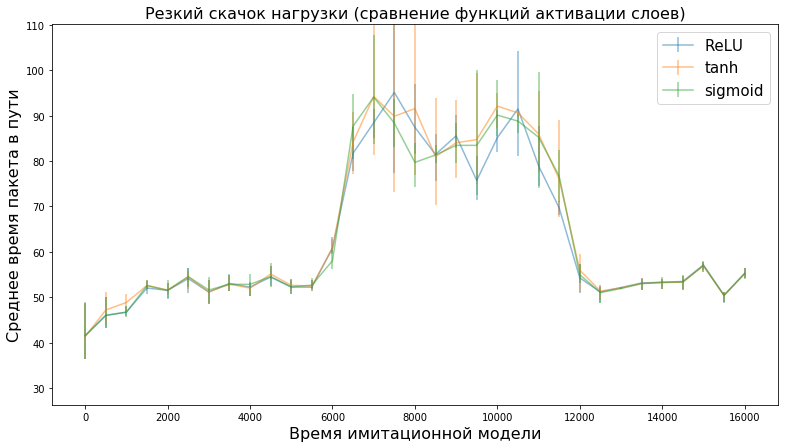
\includegraphics[scale=0.6]{experiment-activations-launch}
\end{figure}

Таким образом, наилучшим алгоритмом оптимизации для данной задачи оказался
RMSProp, а наилучшей функцией активации --- tanh.

\section{Выбор конфигурации feed-forward нейросети}

Было проведено сравнение трех конфигураций feed-forward нейросетей по качеству
предобучения: 2 слоя по 64 нейрона, 2 по 32 и 3 по 32.

\begin{figure}[!h]
  \caption{Сравнение конфигураций feed-forward нейросети по качеству
    предобучения}\label{experiment-layers-pretrain}
  \centering
  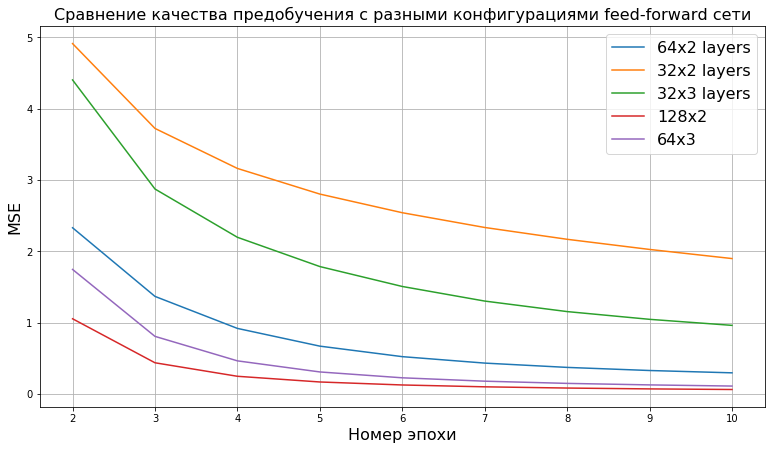
\includegraphics[scale=0.6]{experiment-layers-pretrain}
\end{figure}

\begin{figure}[!h]
  \caption{Сравнение конфигураций feed-forward нейросети по эффективности работы
    в имитационной модели}\label{experiment-layers-launch}
  \centering
  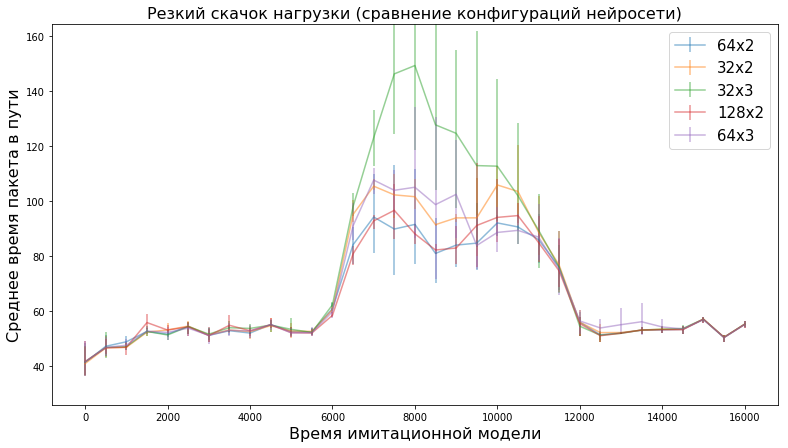
\includegraphics[scale=0.6]{experiment-layers-launch}
\end{figure}

График \ref{experiment-layers-pretrain} показывает, что качество предобучения
растет с повышением количества нейронов. Однако на графике
\ref{experiment-layers-launch} видно, что для способности нейросети
адаптироваться под изменяющиеся условия в сети это неверно: конфигурация с двумя
слоями по 64 нейрона работает лучше, чем конфигурация с тремя слоями по 64
нейрона, и столь же хорошо, как и конфигурация с двумя слоями по 128 нейронов. В
итоге среди двух наиболее успешных конфигураций (64x2 и 128x2) была выбрана
конфигурация 64x2 как менее требовательная к вычислительной мощности.

\section{Исследование влияния softmax-стратегии на работу алгоритма}\label{apx:softmax}

Как указано в разделе \ref{algo:softmax}, для того, чтобы достичь компромисса
между исследованием и использованием, алгоритм DQN-routing использует
softmax-стратегию.

\begin{figure}[!h]
  \caption{Сравнение эффективности алгоритма с использованием softmax-стратегии
    и без}\label{experiment-softmax-effect}
  \centering
  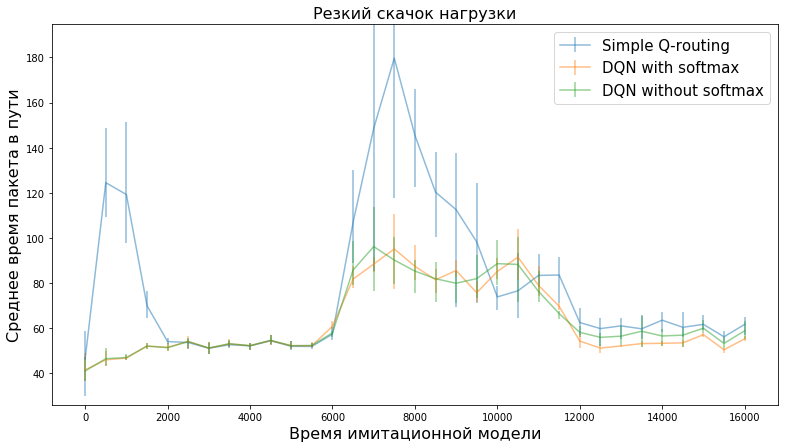
\includegraphics[scale=0.6]{experiment-softmax-effect}
\end{figure}

На графике \ref{experiment-softmax-effect} видно, что алгоритм без использования
softmax-стратегии в сценарии скачка нагрузки в модели компьютерной сети не
всегда способен вернуться к оптимальному решению после снижения нагрузки, в то
время как с ее использованием он к нему всегда возвращается.

\section{Исследование влияния experience replay на работу алгоритма}\label{apx:exp-replay}

Было исследовано влияние применения experience replay на работу алгоритма. Было
проведено сравнение между обычным равномерным experience replay,
приоритизированным experience replay \cite{schaul2015prioritized}, ими же, но с
учетом только последних 32 встреченных эпизодов и работой без
использования experience replay (только с учетом последнего встреченного эпизода).

\begin{figure}[!h]
  \caption{Сравнение эффективности версий алгоритма с использованием различных
    модификаций experience replay}\label{experiments-xp-variants}
  \centering
  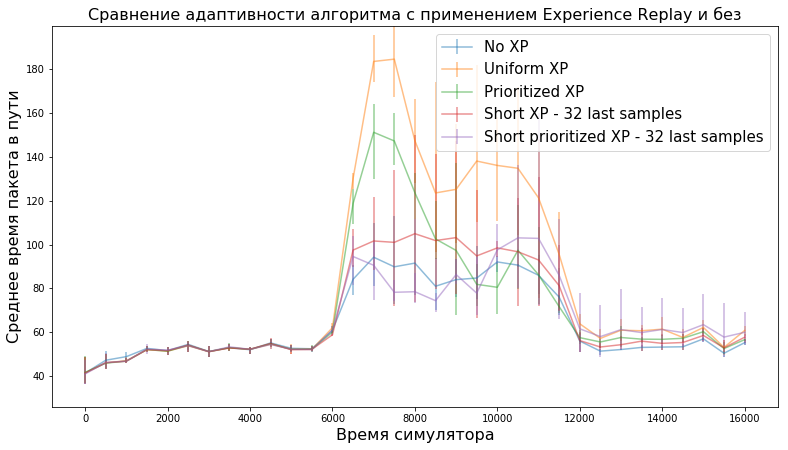
\includegraphics[scale=0.6]{experiments-xp-variants}
\end{figure}

Экспериментально было установлено (\ref{experiments-xp-variants}), что
использование любого вида experience replay отрицательно влияет на способность
алгоритма к адаптации под меняющиеся условия сети, в особенности на способность
сети подстраиваться под снижение нагрузки.

\section{Исследование влияния расширенного состояния на работу алгоритма}\label{apx:amatrix}

Чтобы показать преимущество, получаемое от добавления матрицы смежности на вход
нейросети, было проведено сравнение способности нейросетей с матрицей смежности и
без нее адаптироваться к изменению топологии графа.

\begin{figure}[!h]
  \caption{Сравнение работы DQN с матрицей смежности и без в условиях
    изменяющейся топологии}\label{experiment-with-without-amatrix}
  \centering
  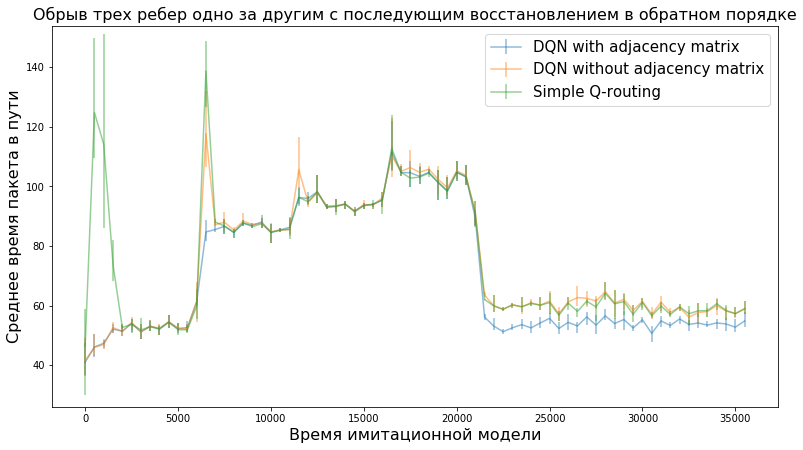
\includegraphics[scale=0.6]{experiment-with-without-amatrix}
\end{figure}

График \ref{experiment-with-without-amatrix} показывает, что нейросети, не
получающие матрицу смежности на вход, не способны вернуться к оптимальному
поведению при восстановлении всех оборванных соединений, и в целом в этом
сценарии показывают поведение аналогичное поведению алгоритма Q-routing.

\begin{figure}[!h]
  \caption{Сравнение работы DQN с информацией о состоянии соседей и без в
    условиях неравномерного потока до выходных вершин, время}\label{experiment-conveyors-en1-time-no-ws}
  \centering
  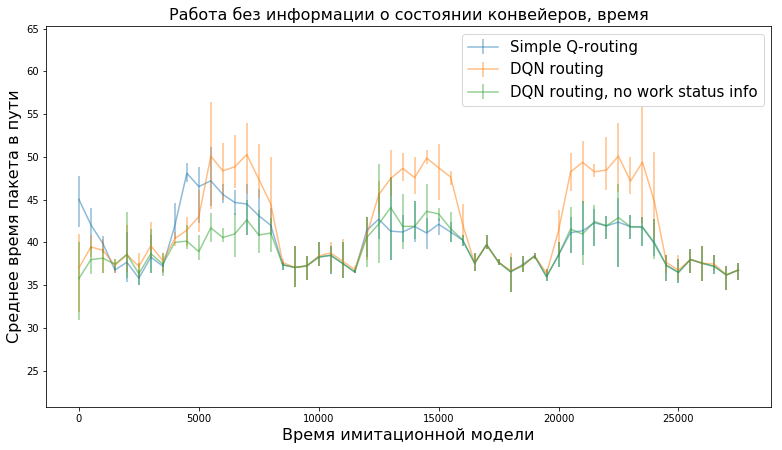
\includegraphics[scale=0.6]{experiment-conveyors-en1-time-no-ws}
\end{figure}

\begin{figure}[!h]
  \caption{Сравнение работы DQN с информацией о состоянии соседей и без в
    условиях неравномерного потока до выходных вершин, время}\label{experiment-conveyors-en1-energy-no-ws}
  \centering
  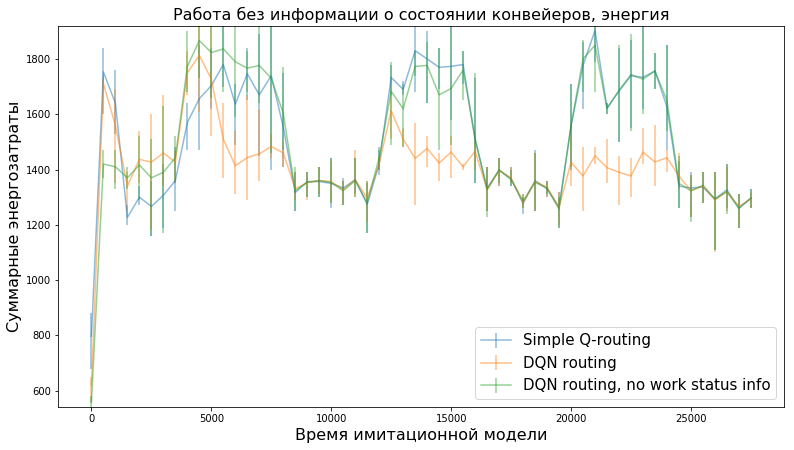
\includegraphics[scale=0.6]{experiment-conveyors-en1-energy-no-ws}
\end{figure}

В сценарии неравномерного потока чемоданов до выходных вершин в конвейерной сети
(\ref{experiments:conveyors/altering-flow})
информация о состояниях соседей (находятся ли они в режиме ожидания или нет)
позволяет точнее предсказывать вознаграждения за действия. На графиках
\ref{experiment-conveyors-en1-time-no-ws} и
\ref{experiment-conveyors-en1-energy-no-ws} видно, что без этой информации
нейросети не способны эффективно оптимизировать энергозатраты и в целом ведут
себя примерно так же, как и обычный Q-routing.

\end{document}
